\documentclass[12pt,a4paper]{article}

% --- Cấu hình Tiếng Việt và Font ---
\usepackage[utf8]{inputenc}
\usepackage[vietnamese]{babel}
\usepackage[T1]{fontenc}
\usepackage{lmodern}

% --- Gói hỗ trợ ---
\usepackage{hyperref}
\usepackage{amssymb}
\usepackage{enumitem}
\usepackage{graphicx}
\usepackage{float}
\usepackage{xcolor}
\usepackage{listings}
\usepackage{listingsutf8}
\usepackage{fancyhdr}
\usepackage{geometry}
\geometry{
    a4paper,
    total={160mm,247mm},
    left=25mm,
    top=25mm,
    headheight=14pt,
}

% --- Cấu hình hyperlinks ---
\hypersetup{
    colorlinks=true,
    linkcolor=blue!60!black,
    urlcolor=blue!70!black,
    citecolor=blue!60!black,
}

% --- Cấu hình listings cho code ---
\definecolor{codebg}{HTML}{F5F5F5}
\definecolor{codeframe}{HTML}{CCCCCC}
\definecolor{codekw}{HTML}{D73A49}
\definecolor{codestr}{HTML}{032F62}
\definecolor{codecom}{HTML}{6A737D}

\lstset{
    backgroundcolor=\color{codebg},
    frame=single,
    rulecolor=\color{codeframe},
    basicstyle=\ttfamily\small,
    keywordstyle=\color{codekw}\bfseries,
    stringstyle=\color{codestr},
    commentstyle=\color{codecom}\itshape,
    breaklines=true,
    showstringspaces=false,
    tabsize=4,
    xleftmargin=8pt,
    xrightmargin=8pt,
    aboveskip=10pt,
    belowskip=10pt,
    extendedchars=true,
    inputencoding=utf8,
    literate=
      {đ}{{\dj}}1
      {Đ}{{\DJ}}1
      {ặ}{{\~a}}1
      {ế}{{\^e}}1
      {ề}{{\`{\^e}}}1
      {ứ}{{\'{u}}}1
}

% --- Header/Footer ---
\pagestyle{fancy}
\fancyhf{}
\fancyhead[L]{\small\textit{PHP Lab02 — CineHub}}
\fancyhead[R]{\small\textit{22110059 — Lê Phạm Hồng Hiển}}
\fancyfoot[C]{\thepage}
\renewcommand{\headrulewidth}{0.4pt}

% =====================================================
\begin{document}

% ===== TRANG BÌA =====
\begin{titlepage}
\begin{center}

\vspace*{1cm}
\textbf{\Large TRƯỜNG ĐẠI HỌC SƯ PHẠM KỸ THUẬT TP.HCM}\\[4pt]
\textbf{\large KHOA CÔNG NGHỆ THÔNG TIN}\\[2cm]

\hrule height 1pt
\vspace{12pt}
{\Huge \textbf{BÁO CÁO THỰC HÀNH}}\\[8pt]
{\LARGE \textbf{Lab02: PHP GET, POST, HEAD, OPTIONS}}\\[12pt]
\hrule height 1pt

\vspace{2cm}

{\Large \textbf{Ứng dụng: CineHub — Đặt Vé Xem Phim Online}}

\vspace{2cm}

\begin{tabular}{ll}
\textbf{Sinh viên:} & Lê Phạm Hồng Hiển \\
\textbf{MSSV:} & 22110059 \\
\textbf{Lớp:} & -- \\
\textbf{GVHD:} & Thầy Tuấn Trần \\
\textbf{Ngày nộp:} & 27/04/2026 \\
\end{tabular}

\vspace{2cm}

\textbf{GitHub Repository:}\\
\url{https://github.com/lphhien112-gif/PHP-}

\vfill
{\large TP. Hồ Chí Minh, Tháng 4/2026}

\end{center}
\end{titlepage}

% ===== MỤC LỤC =====
\tableofcontents
\newpage

% =====================================================
% CÂU 1: XÂY DỰNG ỨNG DỤNG
% =====================================================
\section{Câu 1: Xây dựng ứng dụng CineHub}

\subsection{Giới thiệu ứng dụng}

Em đã chọn xây dựng \textbf{Mini Event Booking App} theo hướng \textbf{hệ thống đặt vé xem phim trực tuyến} — đặt tên là \textbf{CineHub}.

CineHub cho phép người dùng:
\begin{itemize}[noitemsep]
    \item Xem danh sách 10 bộ phim đang chiếu với poster AI, lọc theo thể loại.
    \item Đặt vé xem phim qua booking modal với thông tin đầy đủ.
    \item Kiểm tra toàn bộ RESTful API qua trang \textbf{API Tester} riêng biệt.
\end{itemize}

\subsection{Kiểm tra môi trường}

\begin{itemize}[noitemsep]
    \item \textbf{PHP:} PHP 8.2.12 (chạy qua XAMPP Apache)
    \item \textbf{Composer:} Cài đặt và cấu hình PSR-4 autoload
    \item \textbf{Git:} Quản lý source code, push lên GitHub
    \item \textbf{IDE:} Visual Studio Code
\end{itemize}

\subsection{Cấu trúc dự án}

Dự án tuân thủ chuẩn cấu trúc MVC:

\begin{verbatim}
EventHub/
|-- composer.json          # PSR-4 Autoload
|-- .env                   # Environment variables
|-- .env.example           # Template env
|-- config/
|   `-- app.php            # Read env config
|-- public/
|   |-- index.php          # Entry point (Router)
|   |-- api-tester.html    # API Tester (Postman-style)
|   |-- .htaccess          # Apache rewrite rules
|   `-- assets/
|       |-- css/style.css  # Design system
|       `-- images/        # 10 AI movie posters
|-- src/
|   |-- Controllers/
|   |   `-- EventController.php
|   |-- Helpers/
|   |   `-- ResponseHelper.php
|   `-- Support/
|       `-- Logger.php
|-- views/
|   `-- home.html          # Homepage
`-- storage/logs/
    `-- app.log            # Log file
\end{verbatim}

\subsection{Cấu hình PSR-4 Autoload}

\begin{lstlisting}[caption={composer.json}]
{
    "autoload": {
        "psr-4": {
            "EventHub\\": "src/"
        }
    }
}
\end{lstlisting}

Sau đó chạy lệnh:
\begin{lstlisting}[language=bash]
composer dump-autoload
\end{lstlisting}

\subsection{Cấu hình môi trường (.env)}

\begin{lstlisting}[caption={.env}]
APP_NAME=CineHub
APP_ENV=development
APP_DEBUG=true
\end{lstlisting}

File \texttt{config/app.php} đọc biến môi trường qua hàm \texttt{parse\_ini\_file()}.

\subsection{Dữ liệu mẫu}

Dữ liệu lưu dưới dạng \textbf{array PHP} trong \texttt{EventController.php} gồm \textbf{10 bộ phim} với đầy đủ thông tin:

\begin{lstlisting}[language=PHP,caption={Ví dụ một bản ghi phim}]
[
    'id'       => 1,
    'title'    => 'Stellar Frontier',
    'category' => 'Sci-Fi',
    'date'     => '2026-05-15',
    'time'     => '19:30',
    'location' => 'CGV Vincom Center, Q.1, TP.HCM',
    'price'    => 120000,
    'capacity' => 150,
    'booked'   => 42,
    'status'   => 'Open',
    'image'    => 'stellar-frontier.png',
    'rating'   => '8.5',
    'director' => 'Christopher Nolan',
]
\end{lstlisting}

10 thể loại phim: Sci-Fi, Romance, Horror, Animation, Action, Crime, Drama, Adventure, Comedy, Documentary.

\subsection{Trang chủ — Giao diện đặt vé}

Trang chủ thiết kế theo phong cách \textbf{dark-mode premium} tương tự CGV/Lotte Cinema, với:
\begin{itemize}[noitemsep]
    \item Hero section với thống kê (suất chiếu, đang bán, ghế trống)
    \item Lưới 10 poster phim AI với badge trạng thái, rating, giá vé
    \item Filter theo 10 thể loại
    \item Booking modal với preview phim (thumbnail + rạp + giá)
    \item Promo banner ưu đãi
\end{itemize}

\begin{figure}[H]
    \centering
    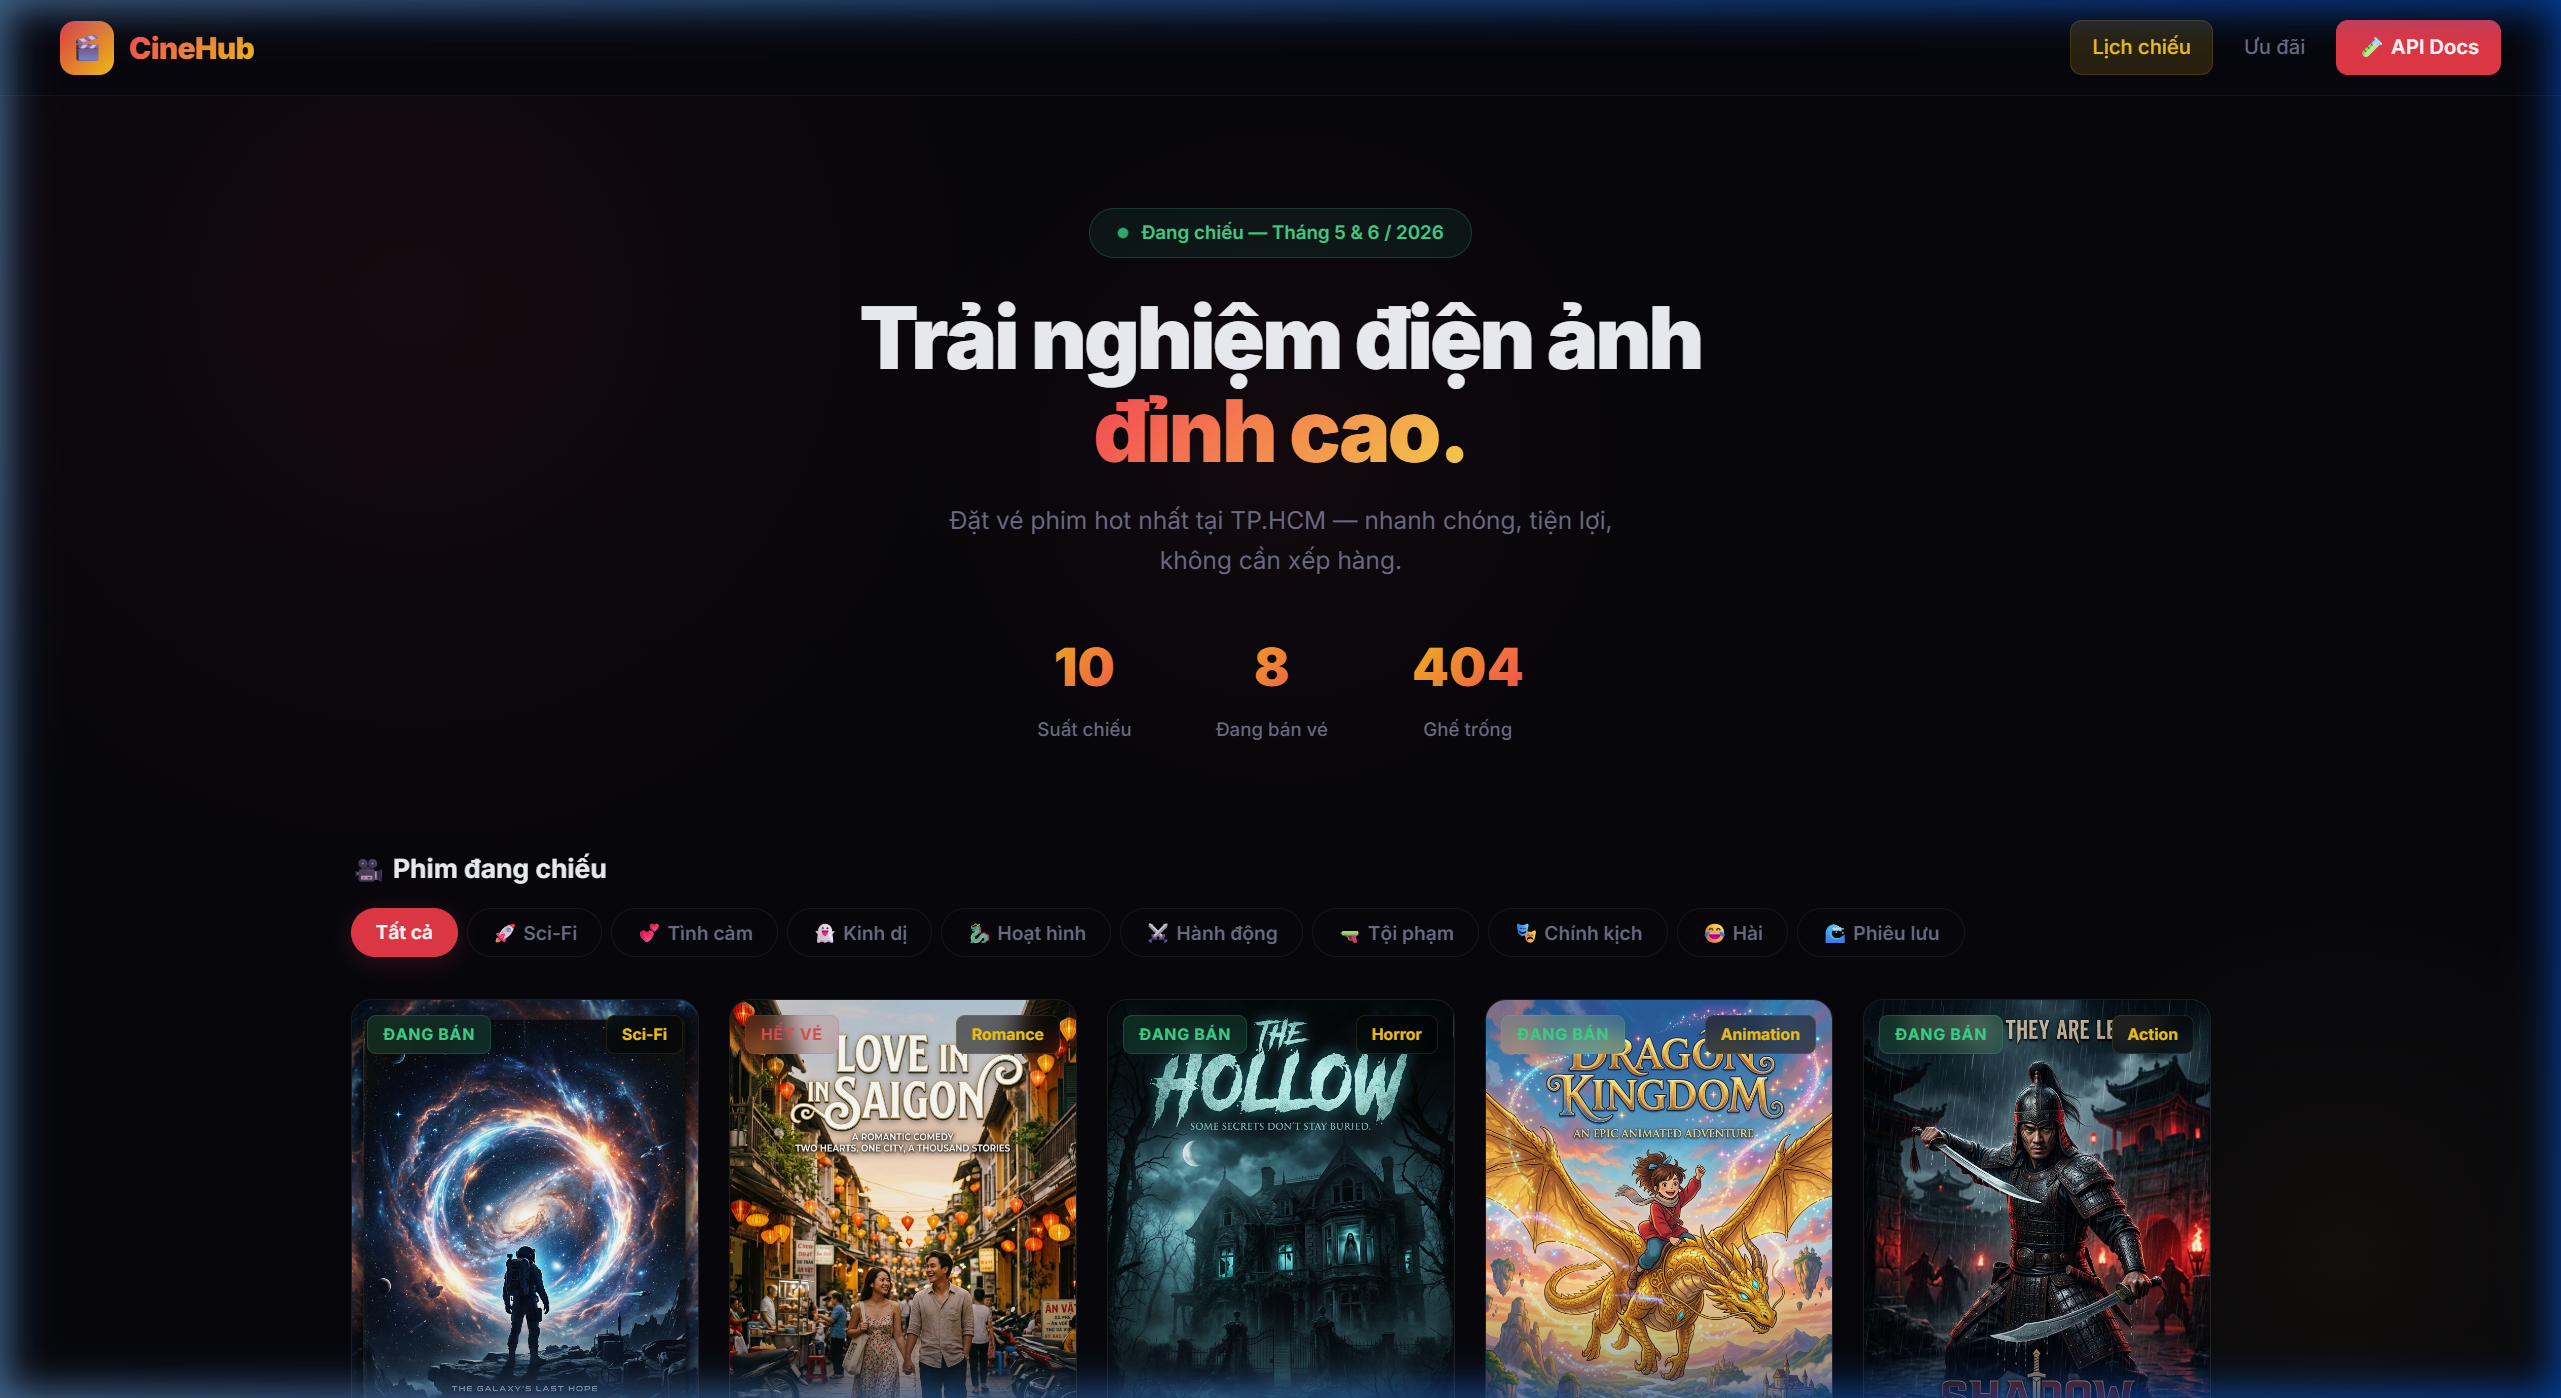
\includegraphics[width=\textwidth]{images/01-homepage.png}
    \caption{Trang chủ CineHub — Hero section và danh sách phim}
\end{figure}

\begin{figure}[H]
    \centering
    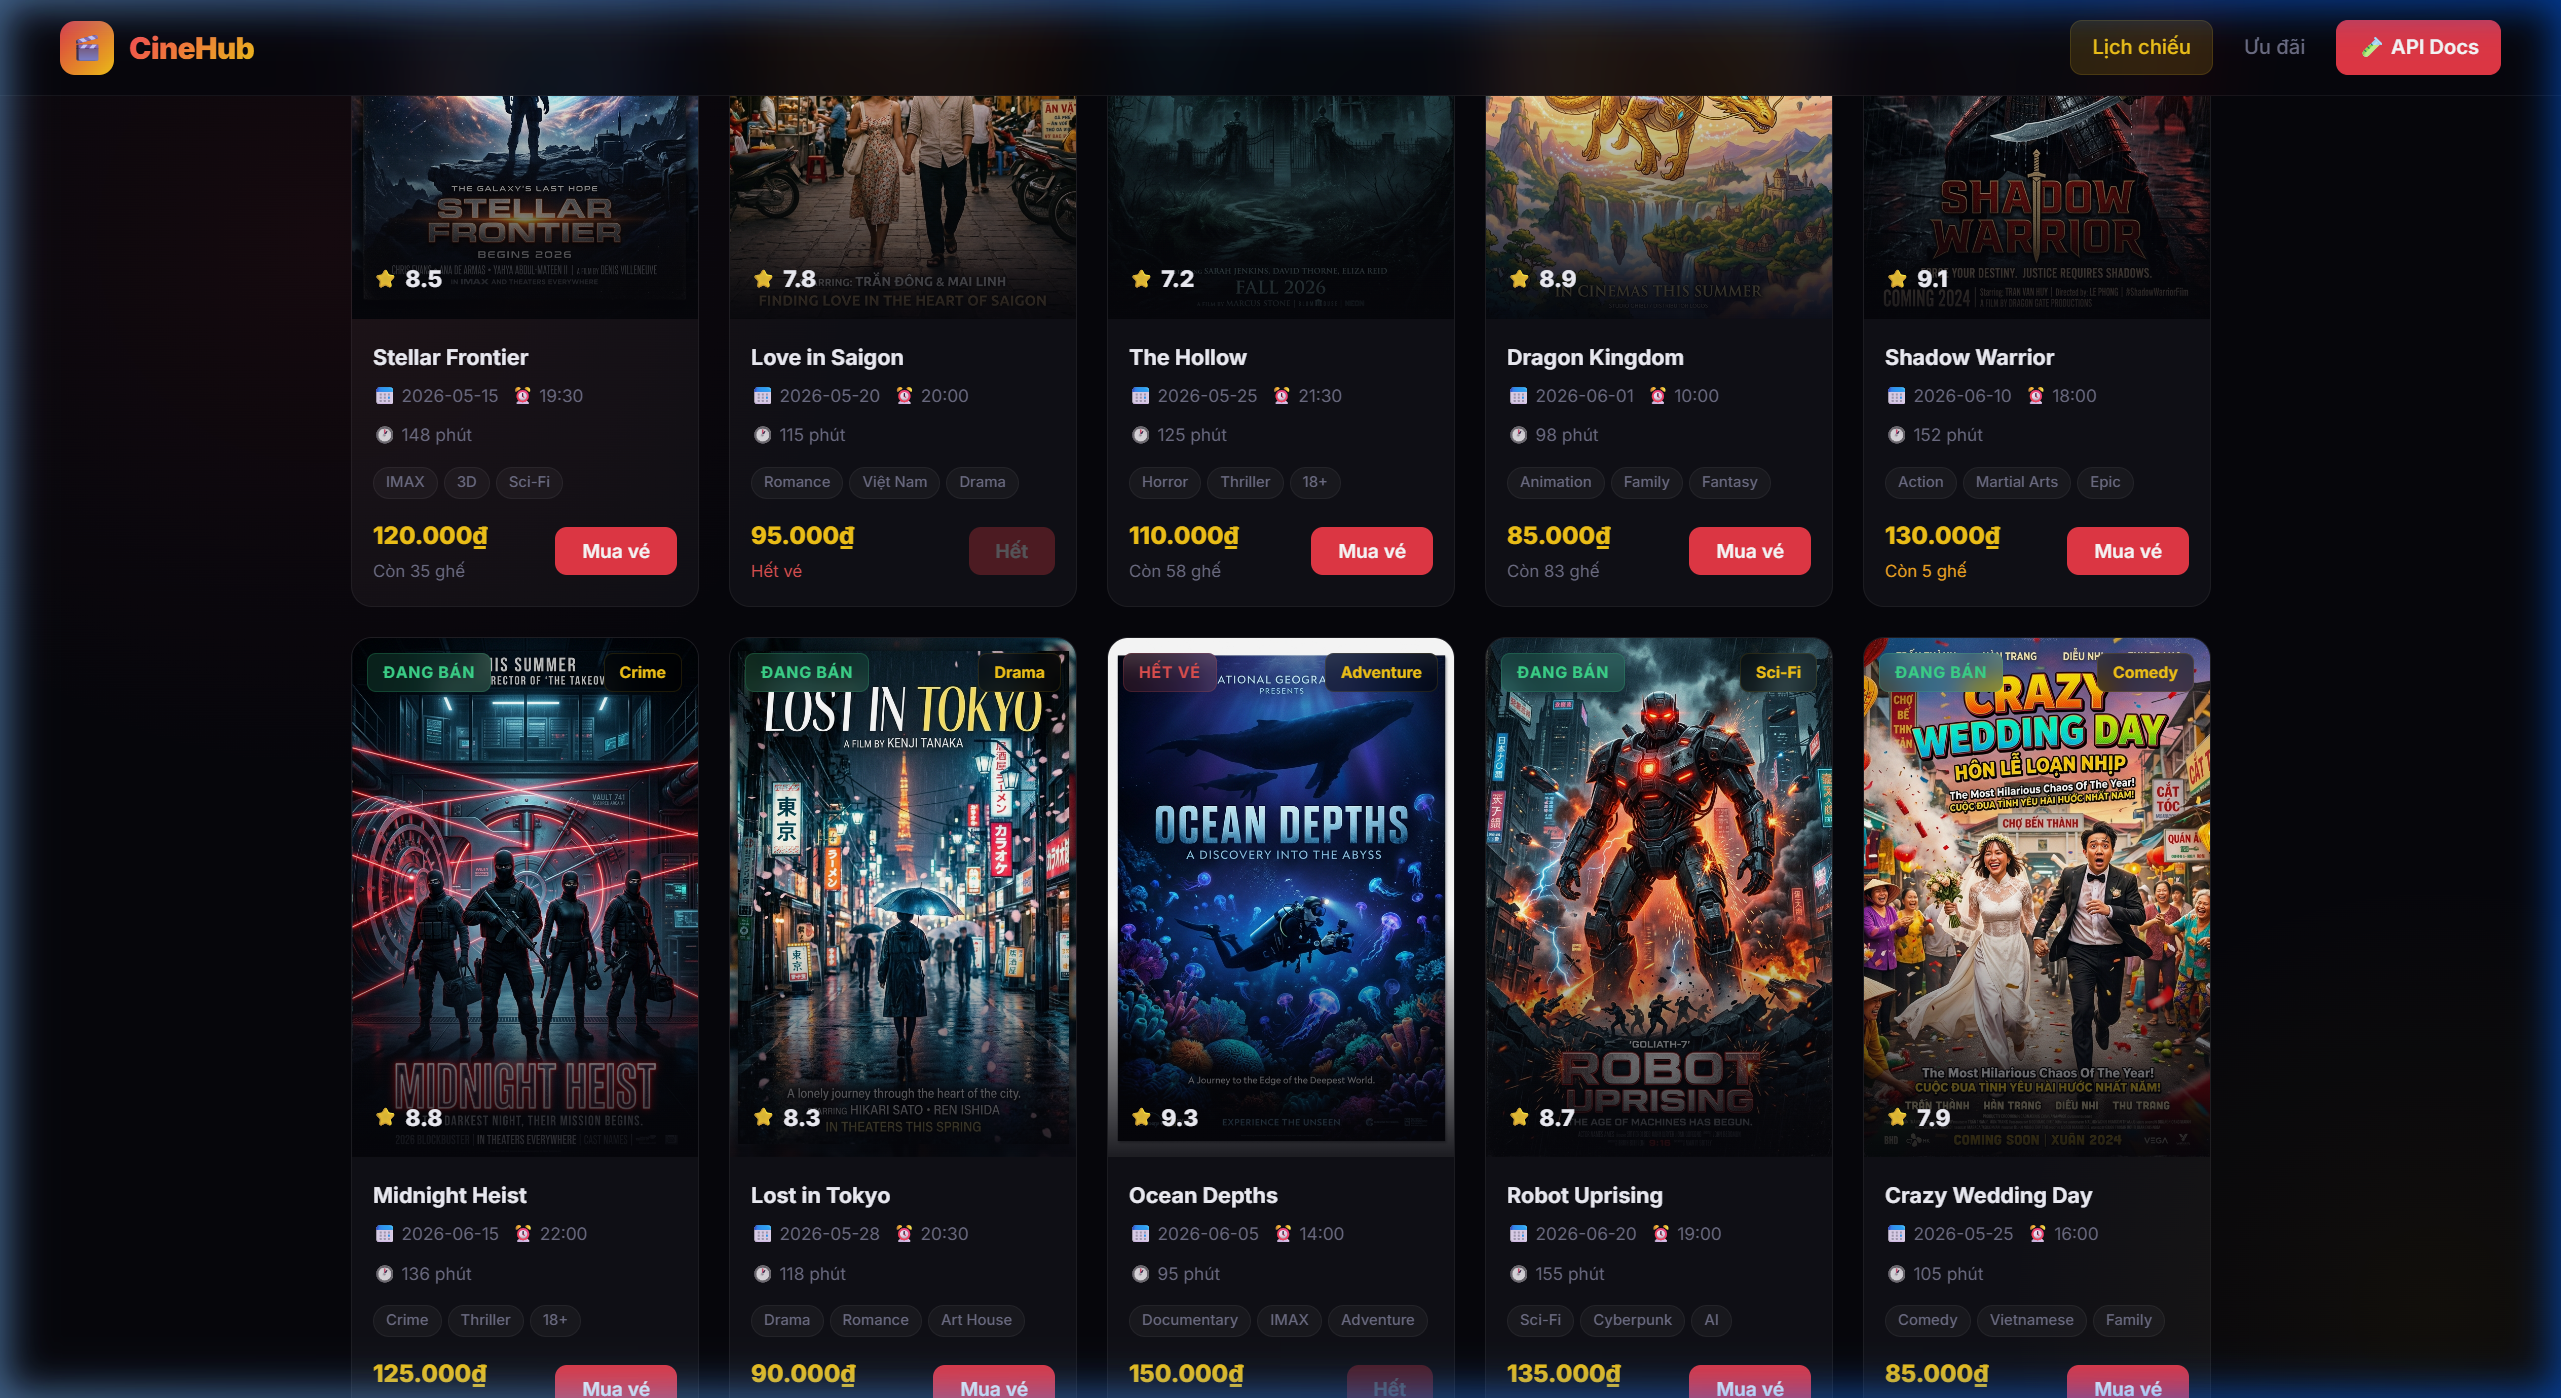
\includegraphics[width=\textwidth]{images/02-promo.png}
    \caption{Promo banner và các phim phía dưới}
\end{figure}

\begin{figure}[H]
    \centering
    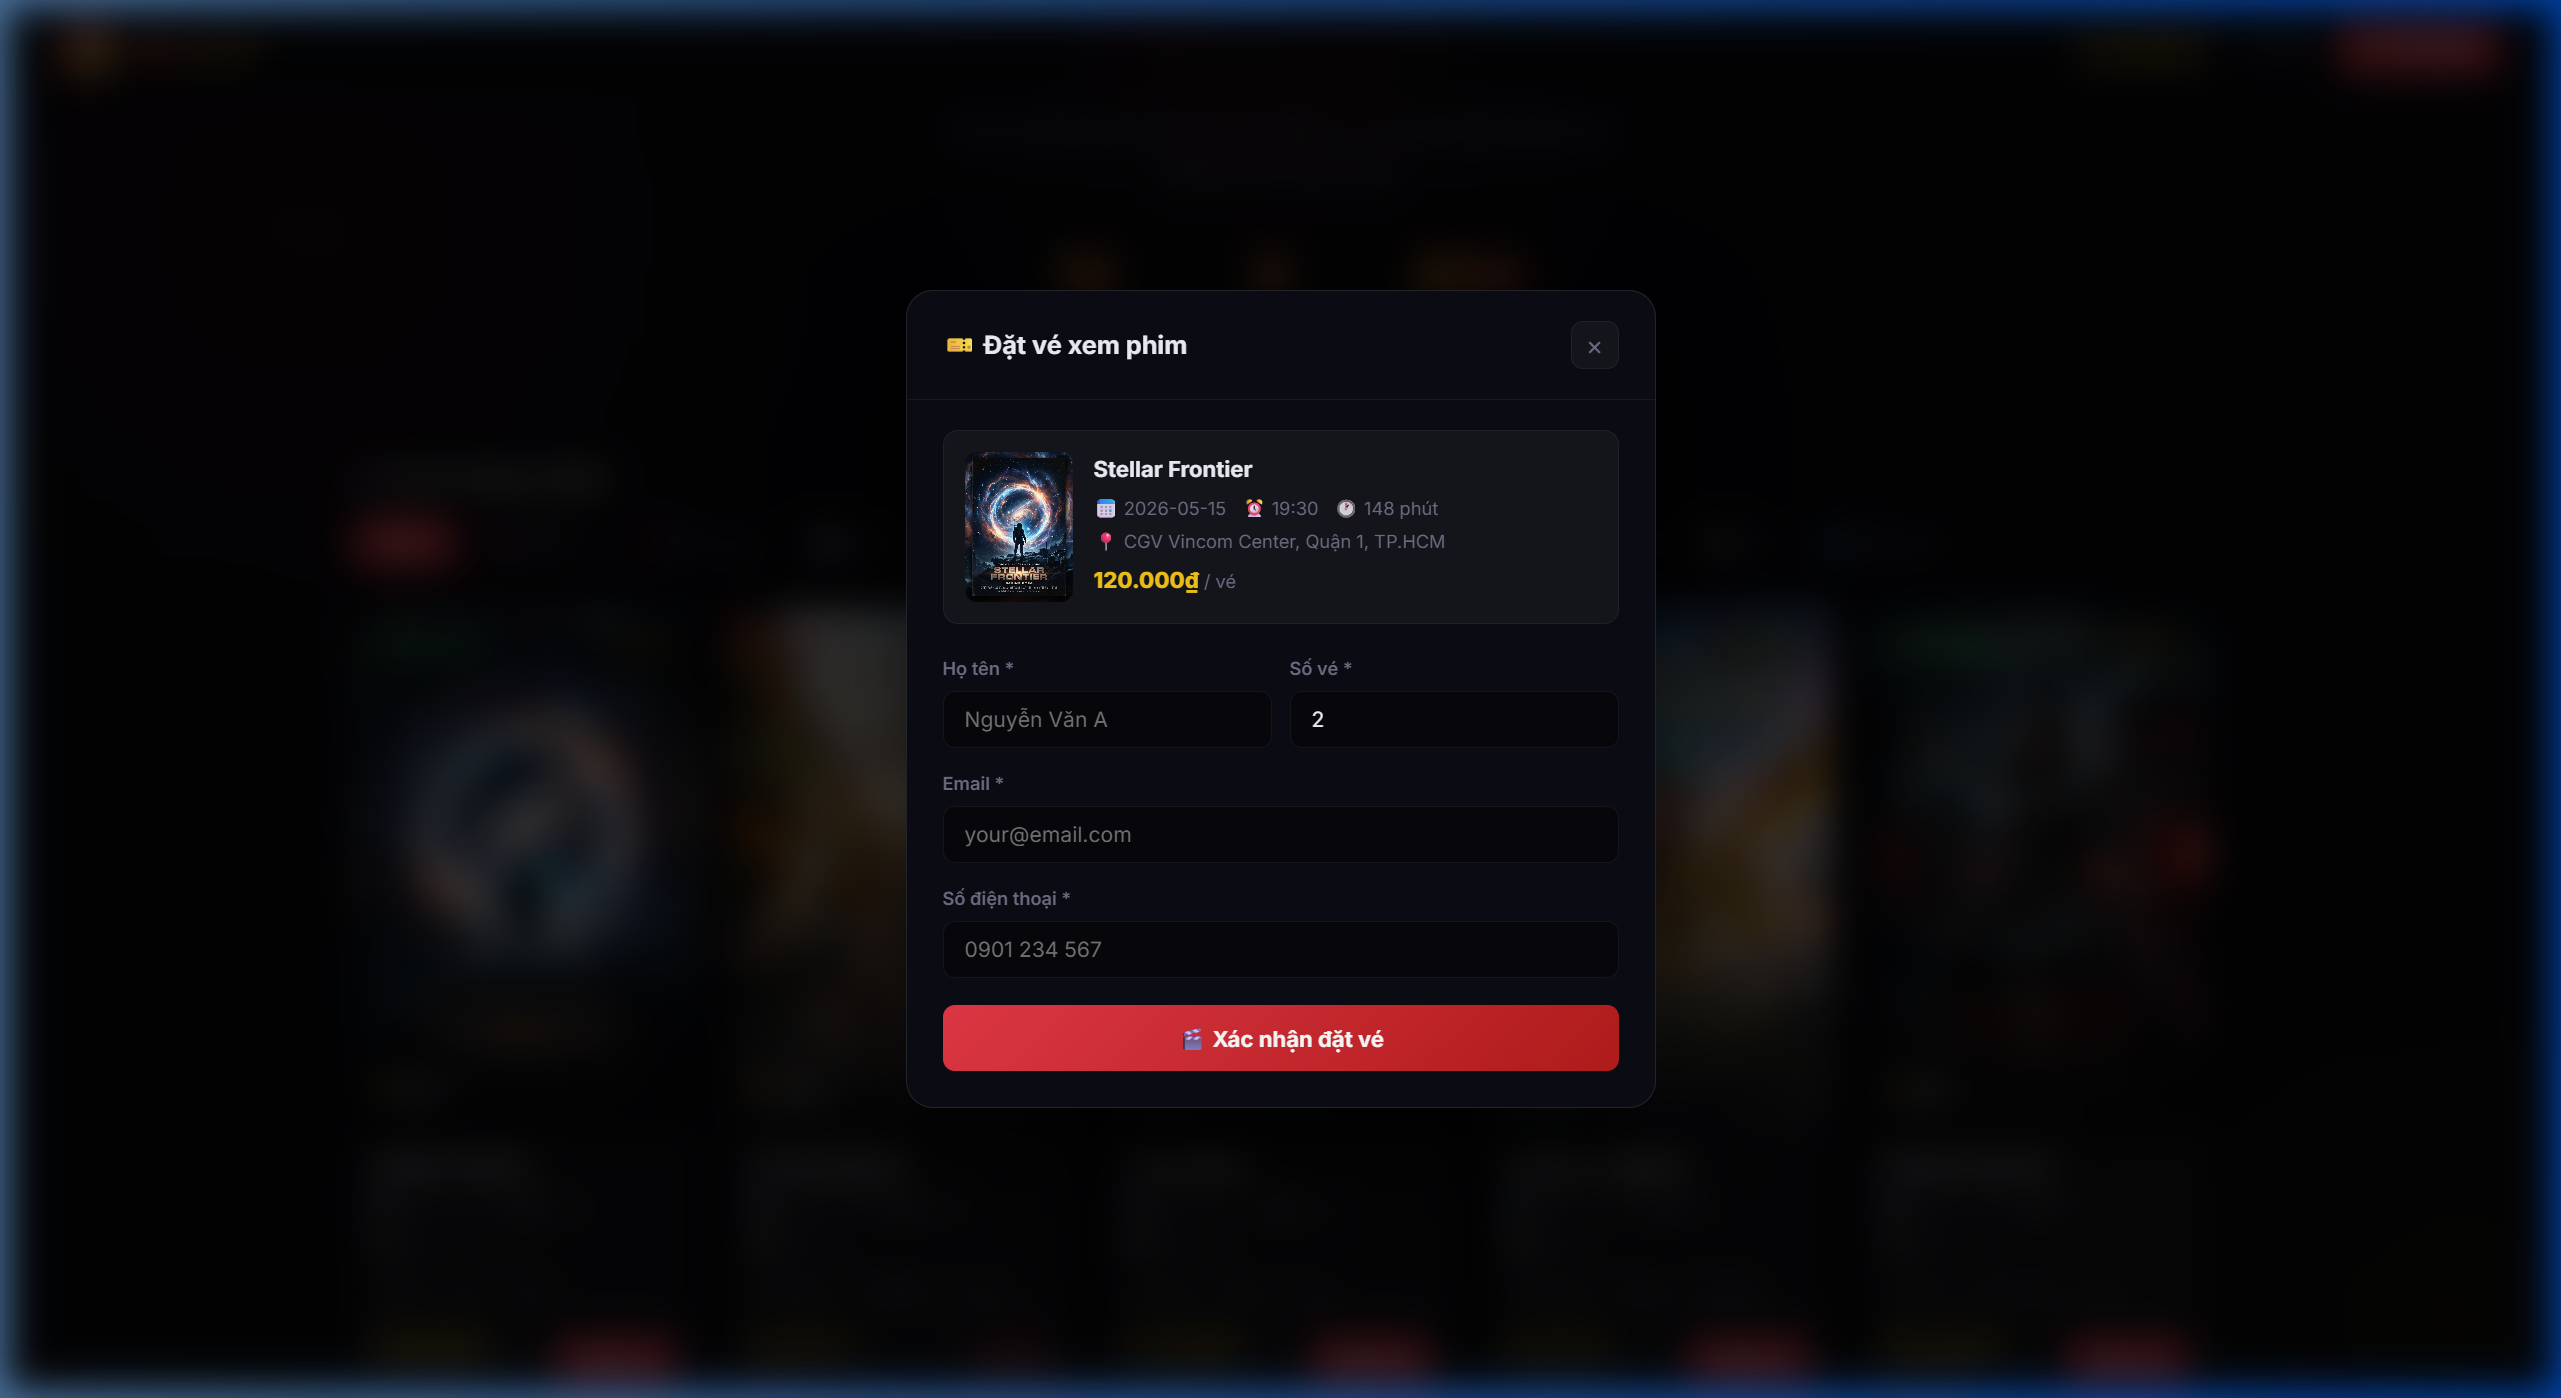
\includegraphics[width=0.7\textwidth]{images/03-booking-modal.png}
    \caption{Booking modal — Preview phim + Form đặt vé}
\end{figure}

\subsection{RESTful API Endpoints}

\subsubsection{GET /events — Danh sách phim (200 OK)}

\begin{lstlisting}[language=bash]
GET /events              -> 200 (danh sach phim)
GET /events?category=Sci-Fi  -> 200 (loc theo the loai)
GET /events/1            -> 200 (chi tiet phim ID=1)
GET /events/999          -> 404 (khong tim thay)
\end{lstlisting}

\begin{figure}[H]
    \centering
    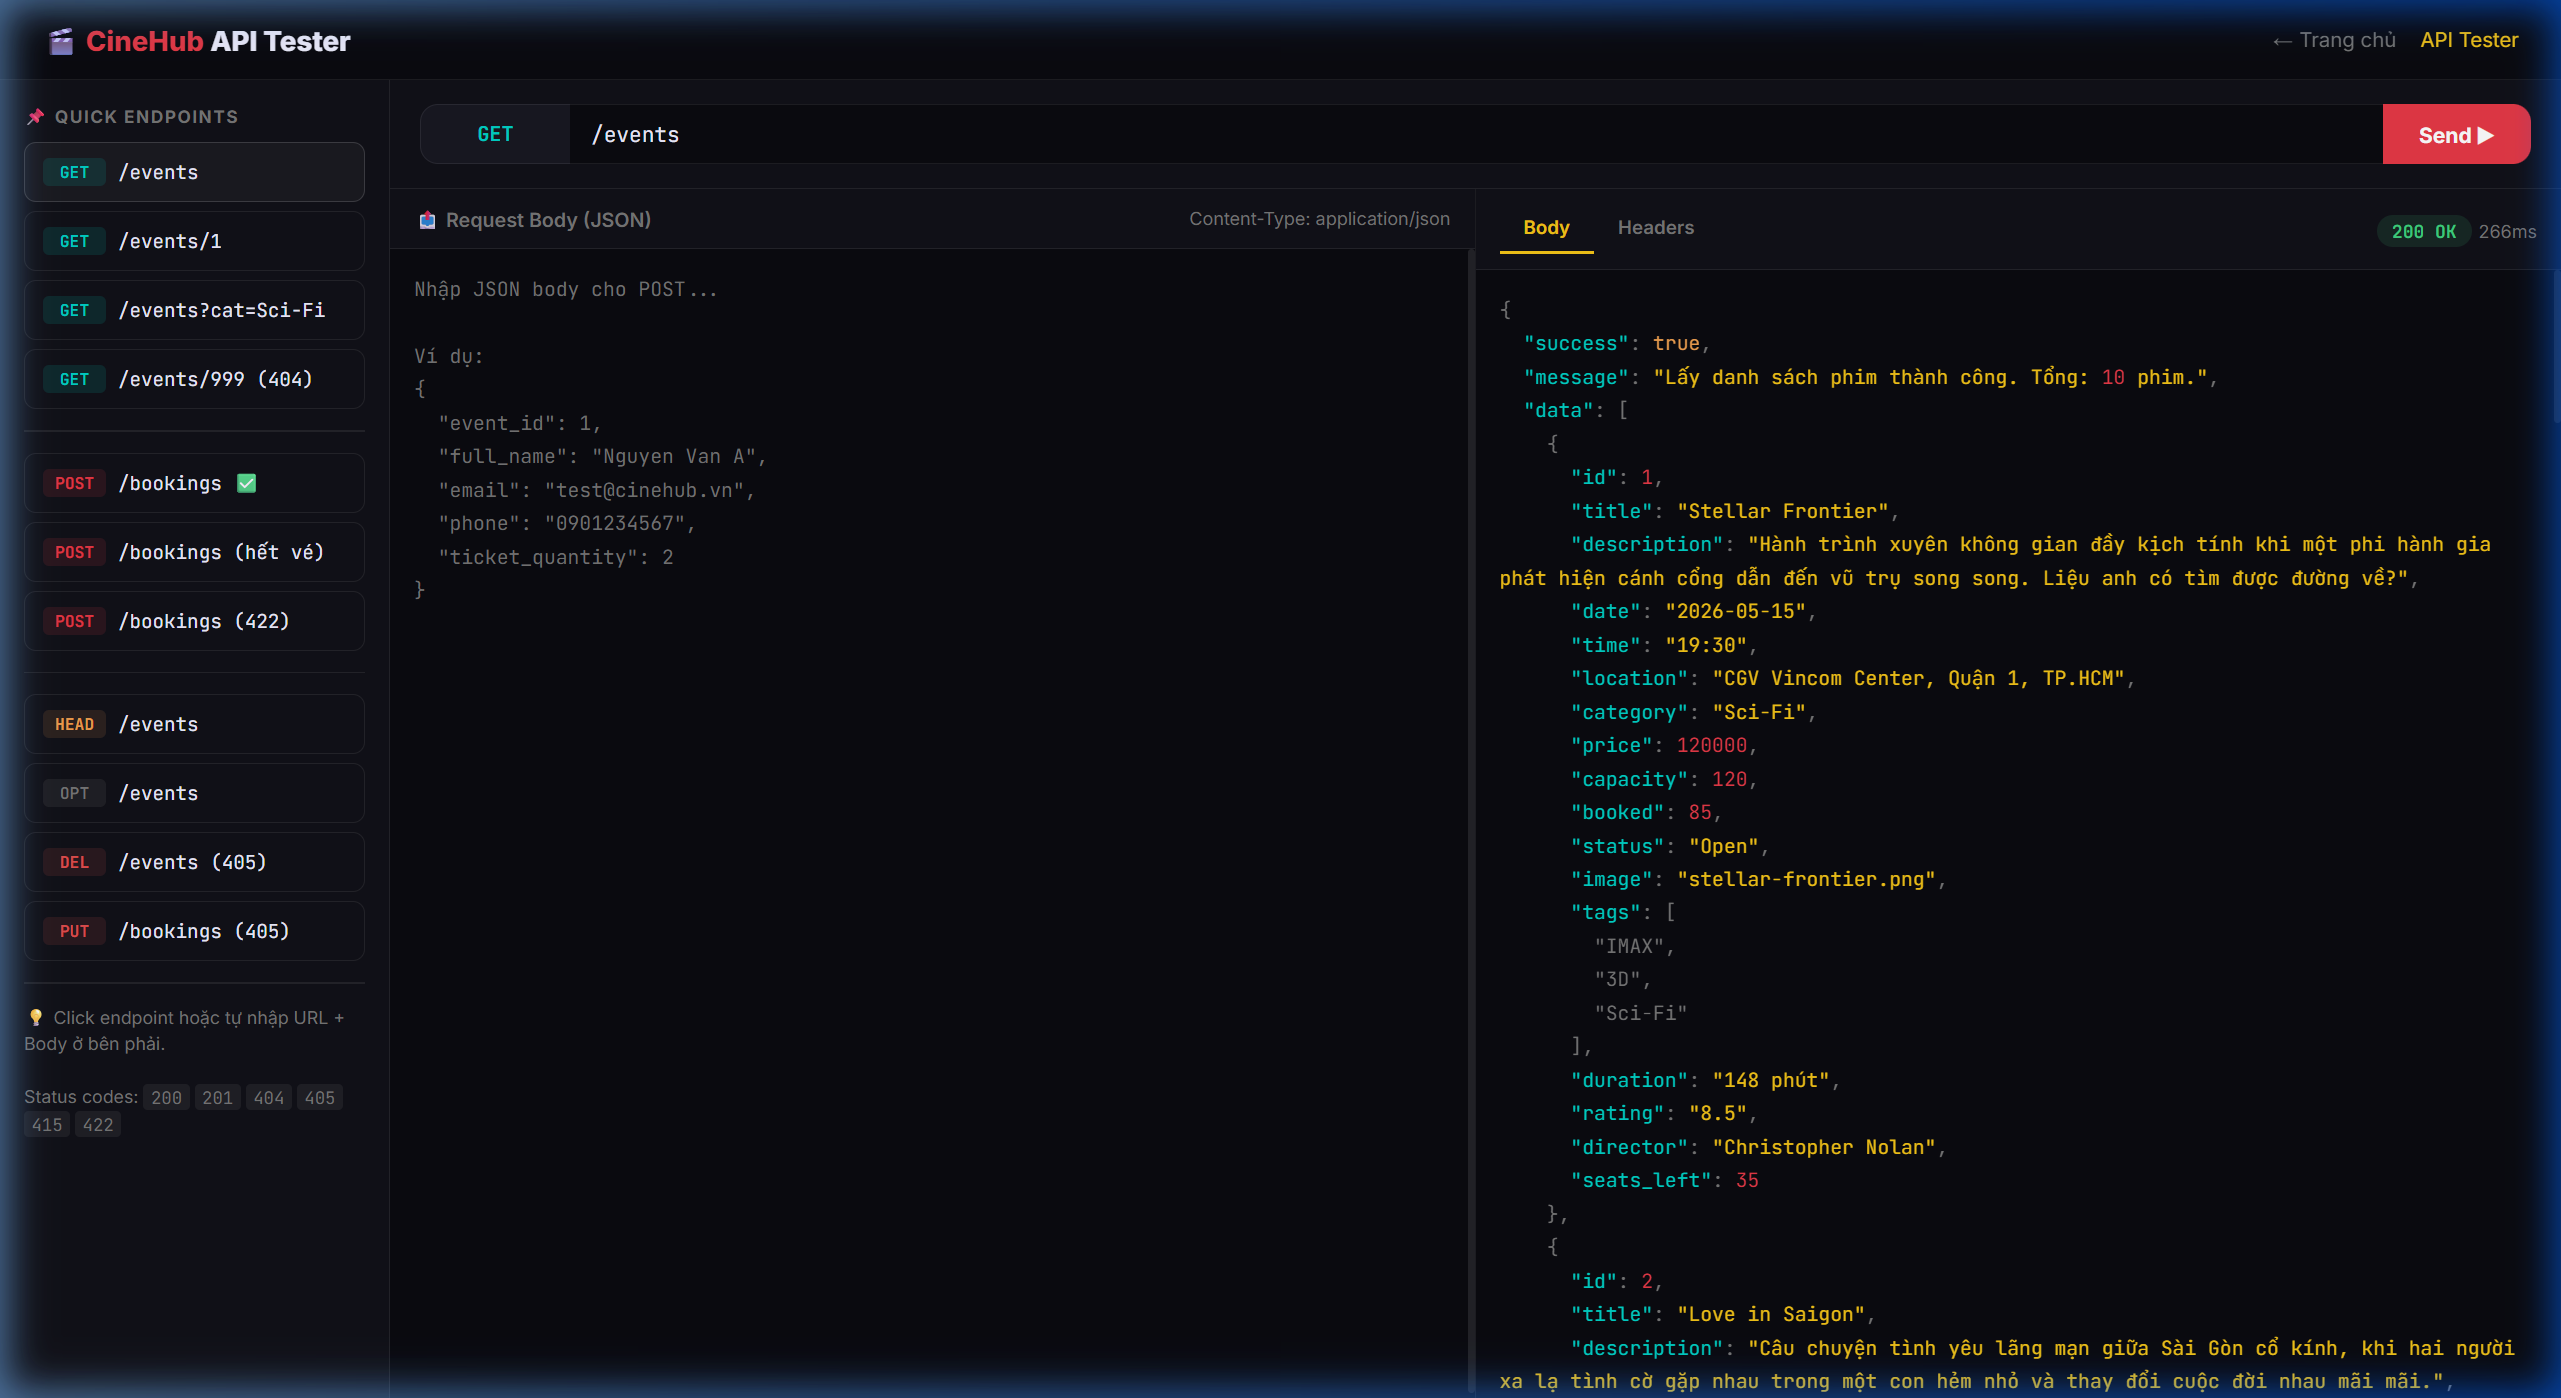
\includegraphics[width=\textwidth]{images/05-get-200.png}
    \caption{GET /events — Trả về 200 OK với danh sách 10 phim}
\end{figure}

\subsubsection{POST /bookings — Đặt vé (201 Created)}

\begin{lstlisting}[caption={Request body}]
{
    "event_id": 1,
    "full_name": "Nguyen Van A",
    "email": "test@cinehub.vn",
    "phone": "0901234567",
    "ticket_quantity": 2
}
\end{lstlisting}

\begin{figure}[H]
    \centering
    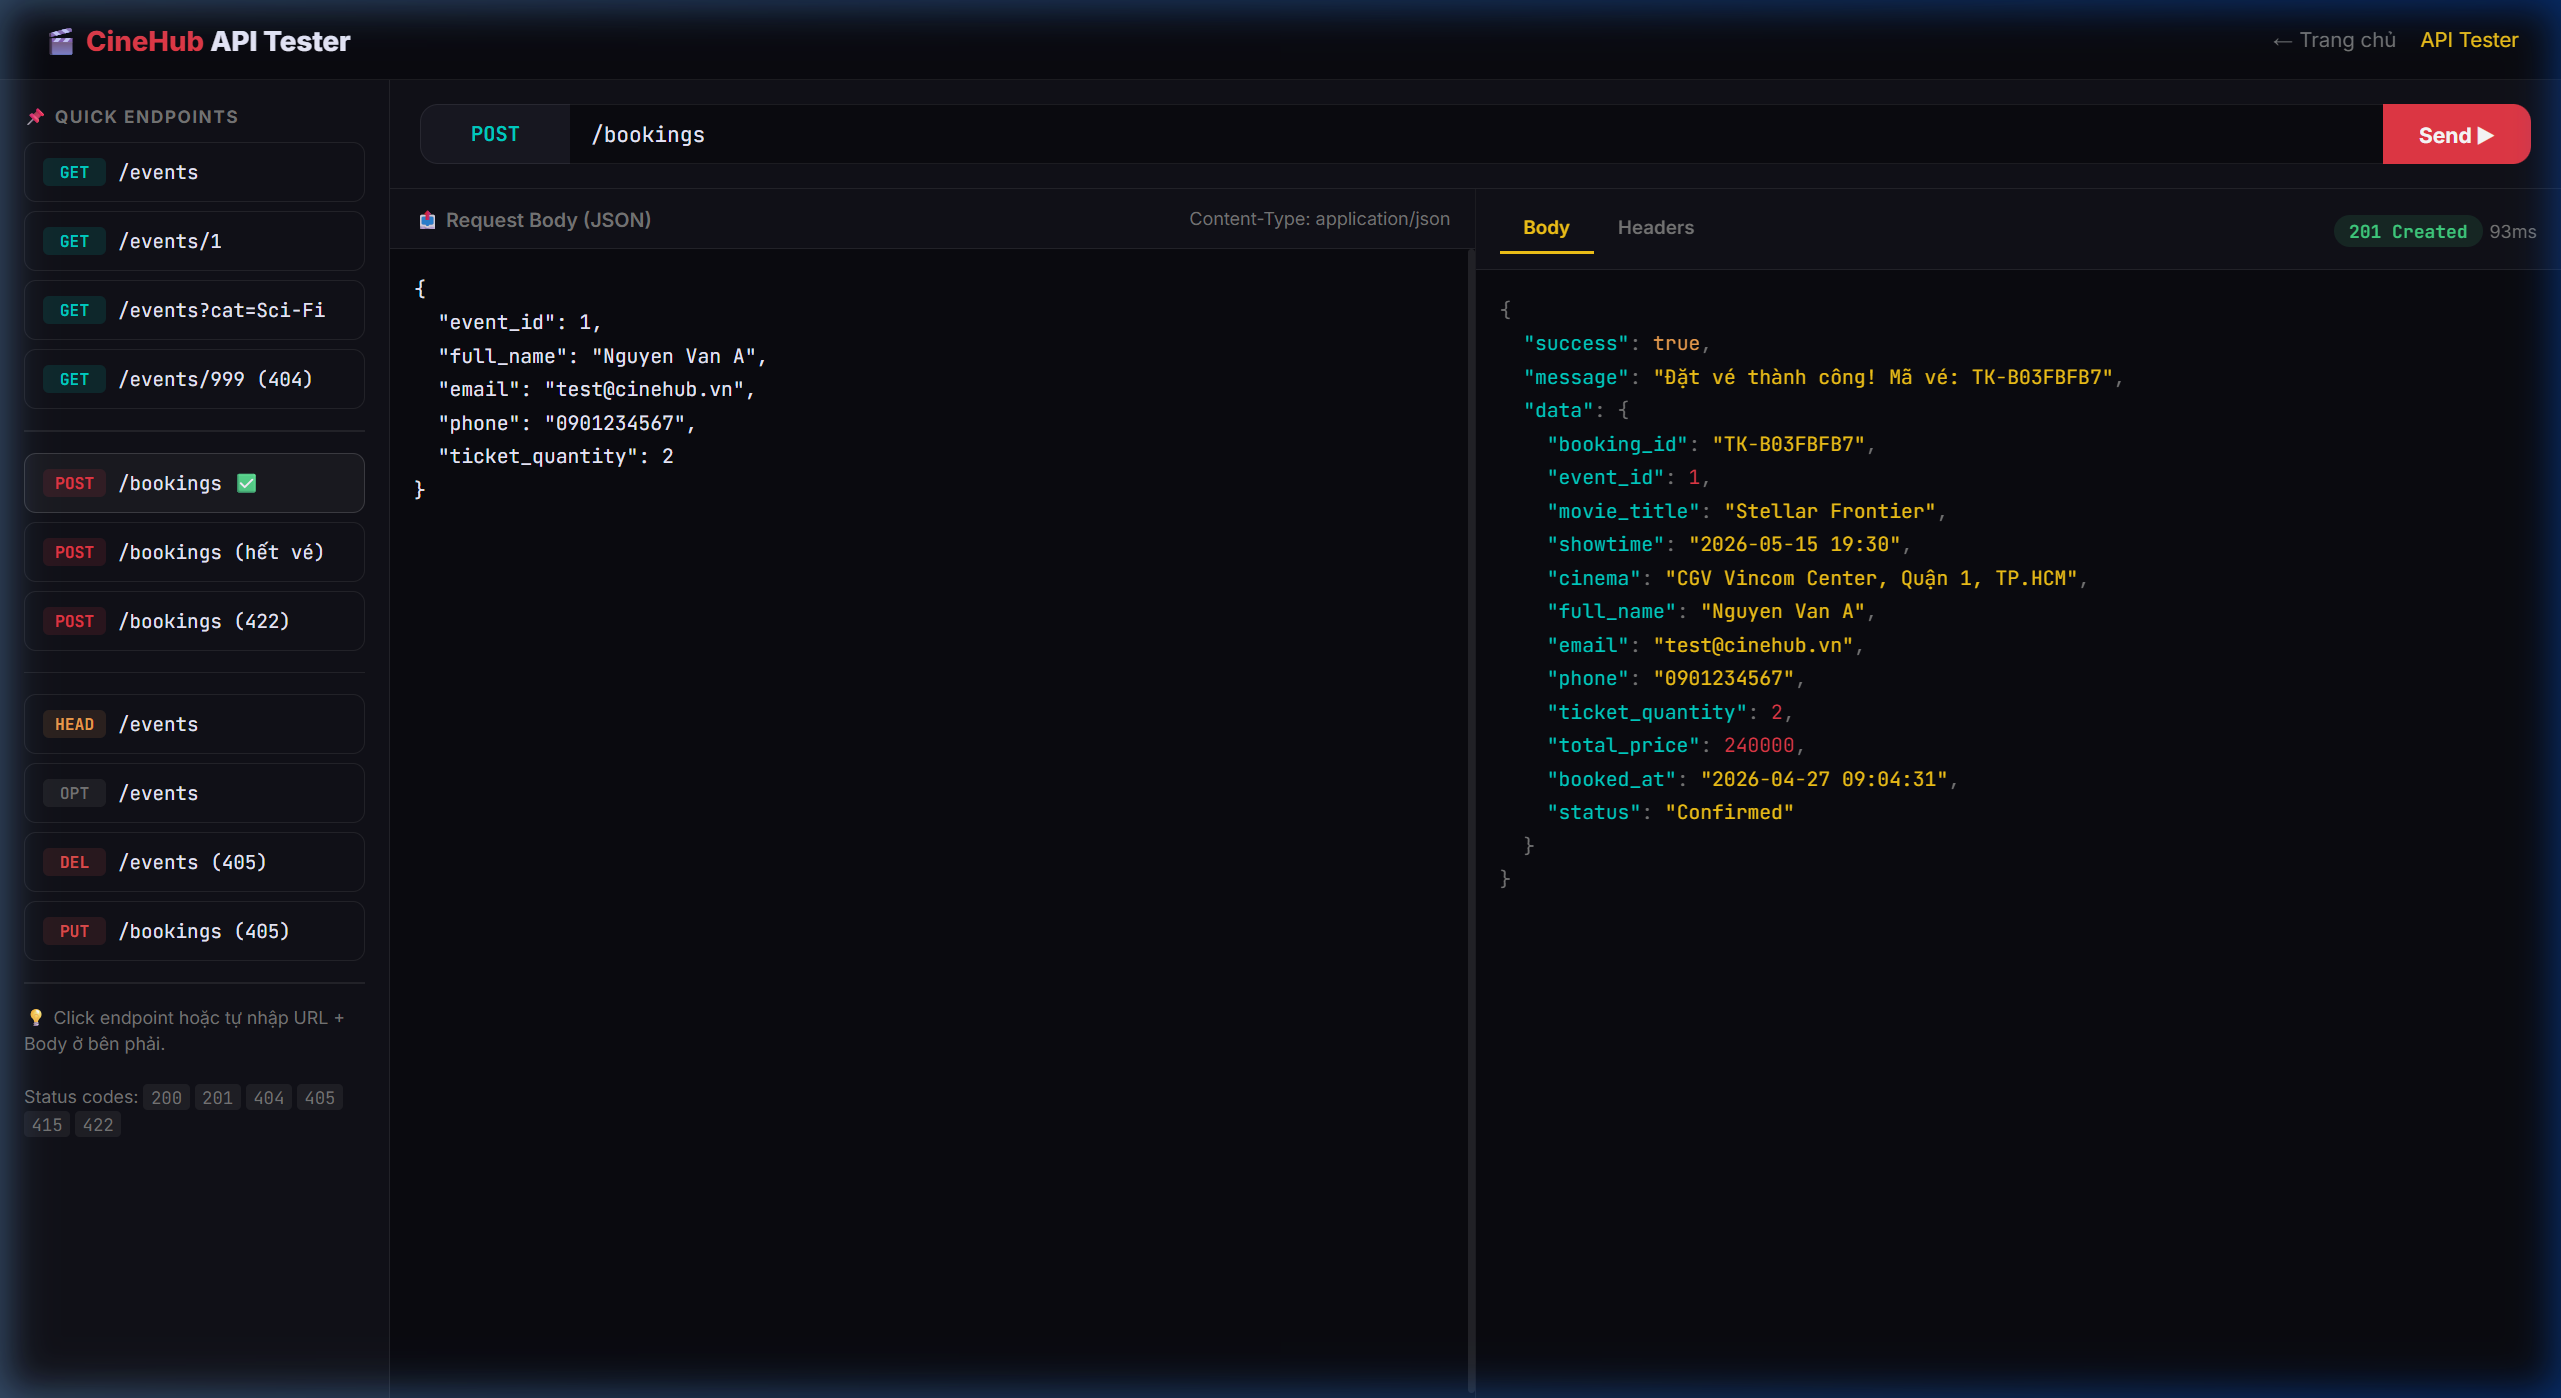
\includegraphics[width=\textwidth]{images/06-post-201.png}
    \caption{POST /bookings — Đặt vé thành công, trả về 201 Created}
\end{figure}

\subsubsection{Xử lý lỗi 404, 405, 415, 422}

\textbf{404 Not Found} — Khi truy cập phim không tồn tại:
\begin{figure}[H]
    \centering
    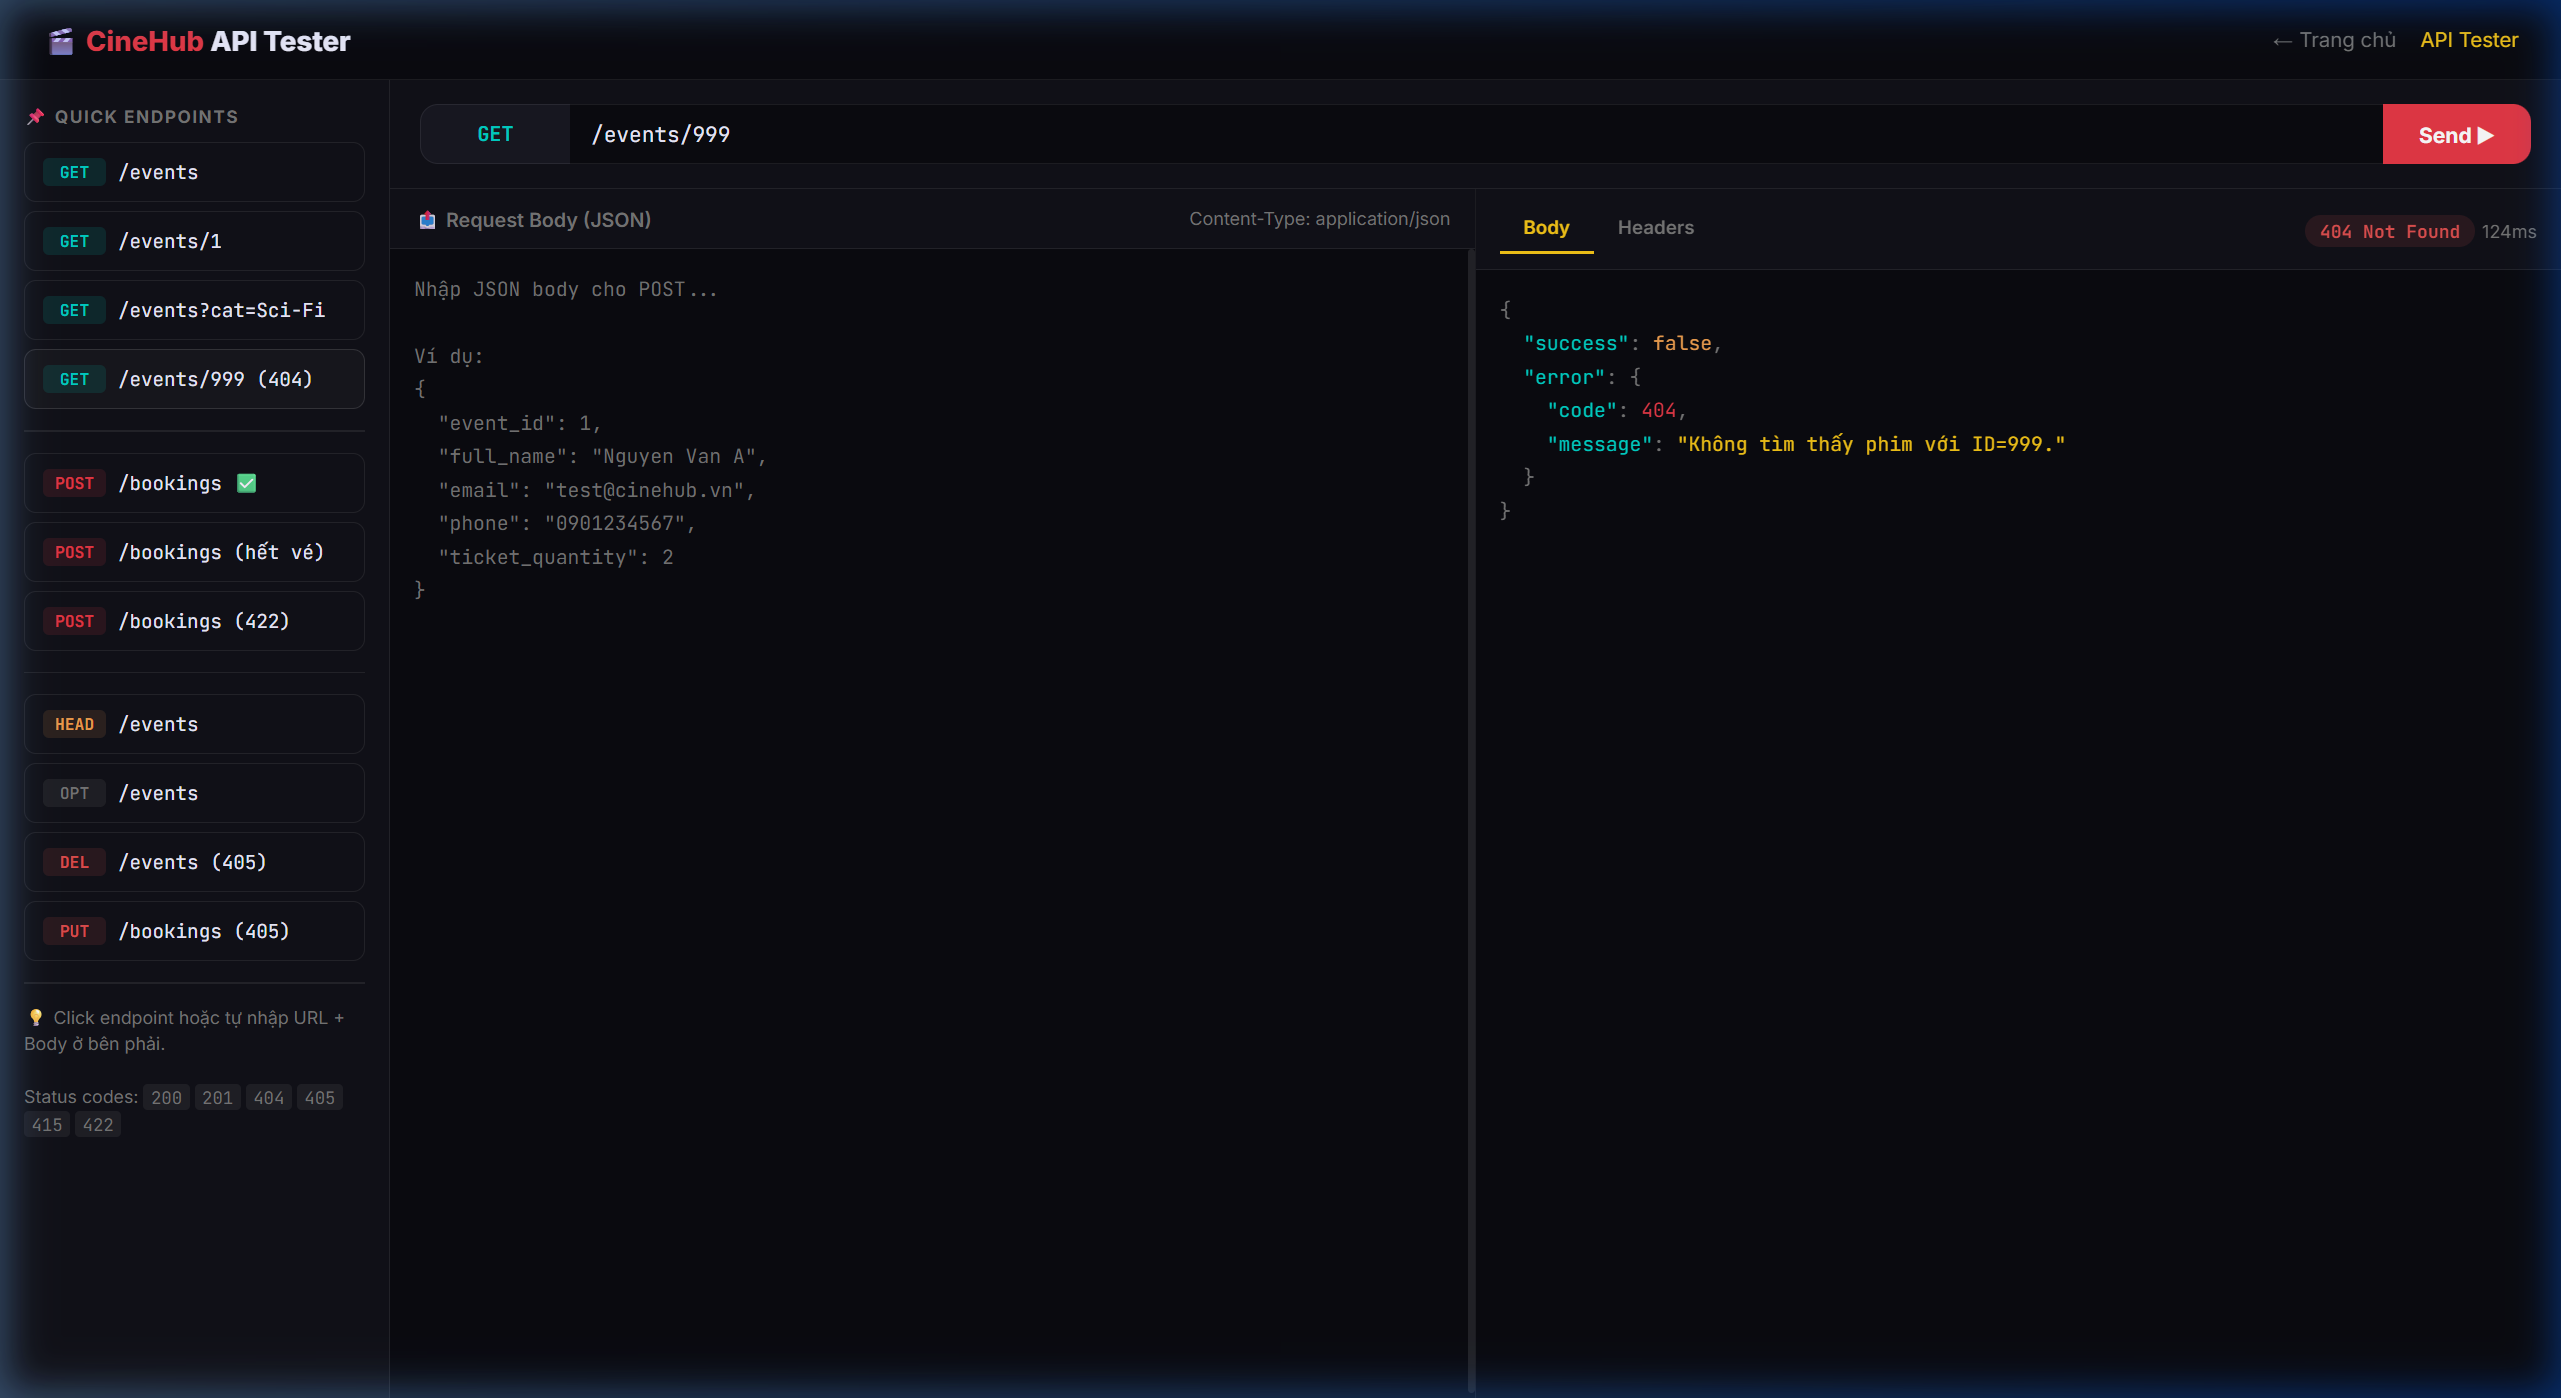
\includegraphics[width=\textwidth]{images/07-get-404.png}
    \caption{GET /events/999 — Trả về 404 Not Found}
\end{figure}

\textbf{422 Unprocessable Entity} — Khi gửi dữ liệu thiếu/sai:
\begin{figure}[H]
    \centering
    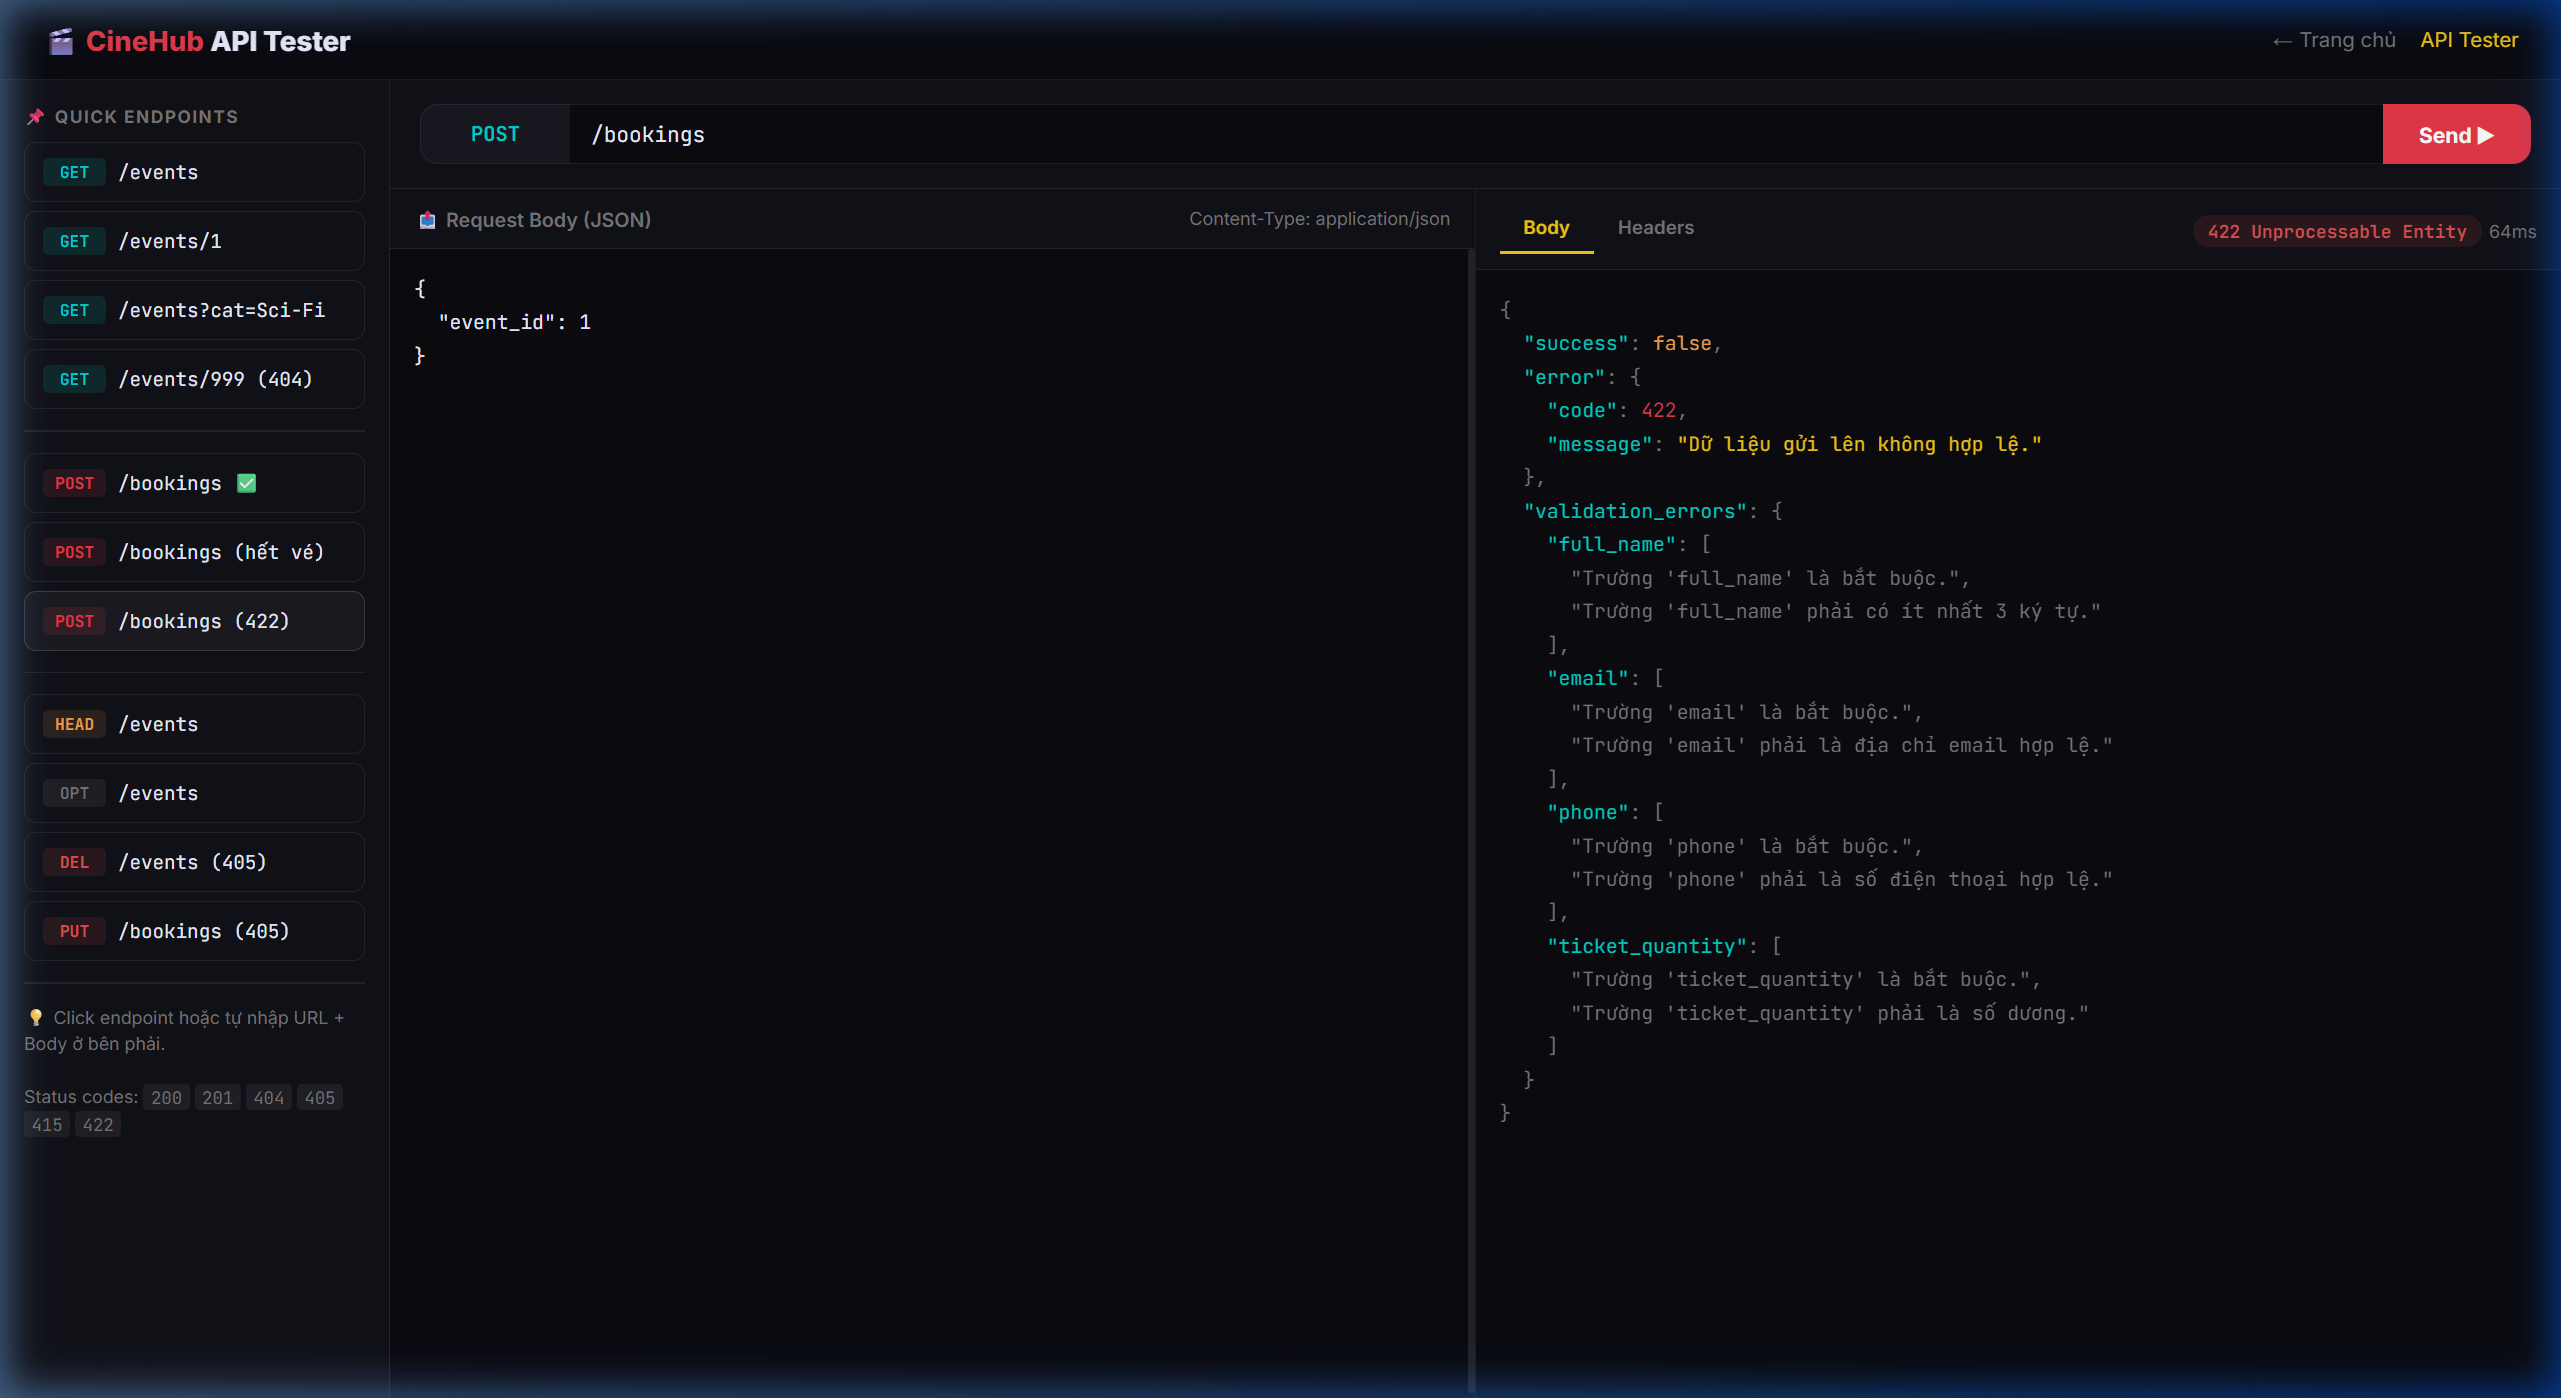
\includegraphics[width=\textwidth]{images/08-post-422.png}
    \caption{POST /bookings thiếu trường — Trả về 422 với danh sách lỗi}
\end{figure}

\textbf{405 Method Not Allowed} — Khi gọi sai method:
\begin{figure}[H]
    \centering
    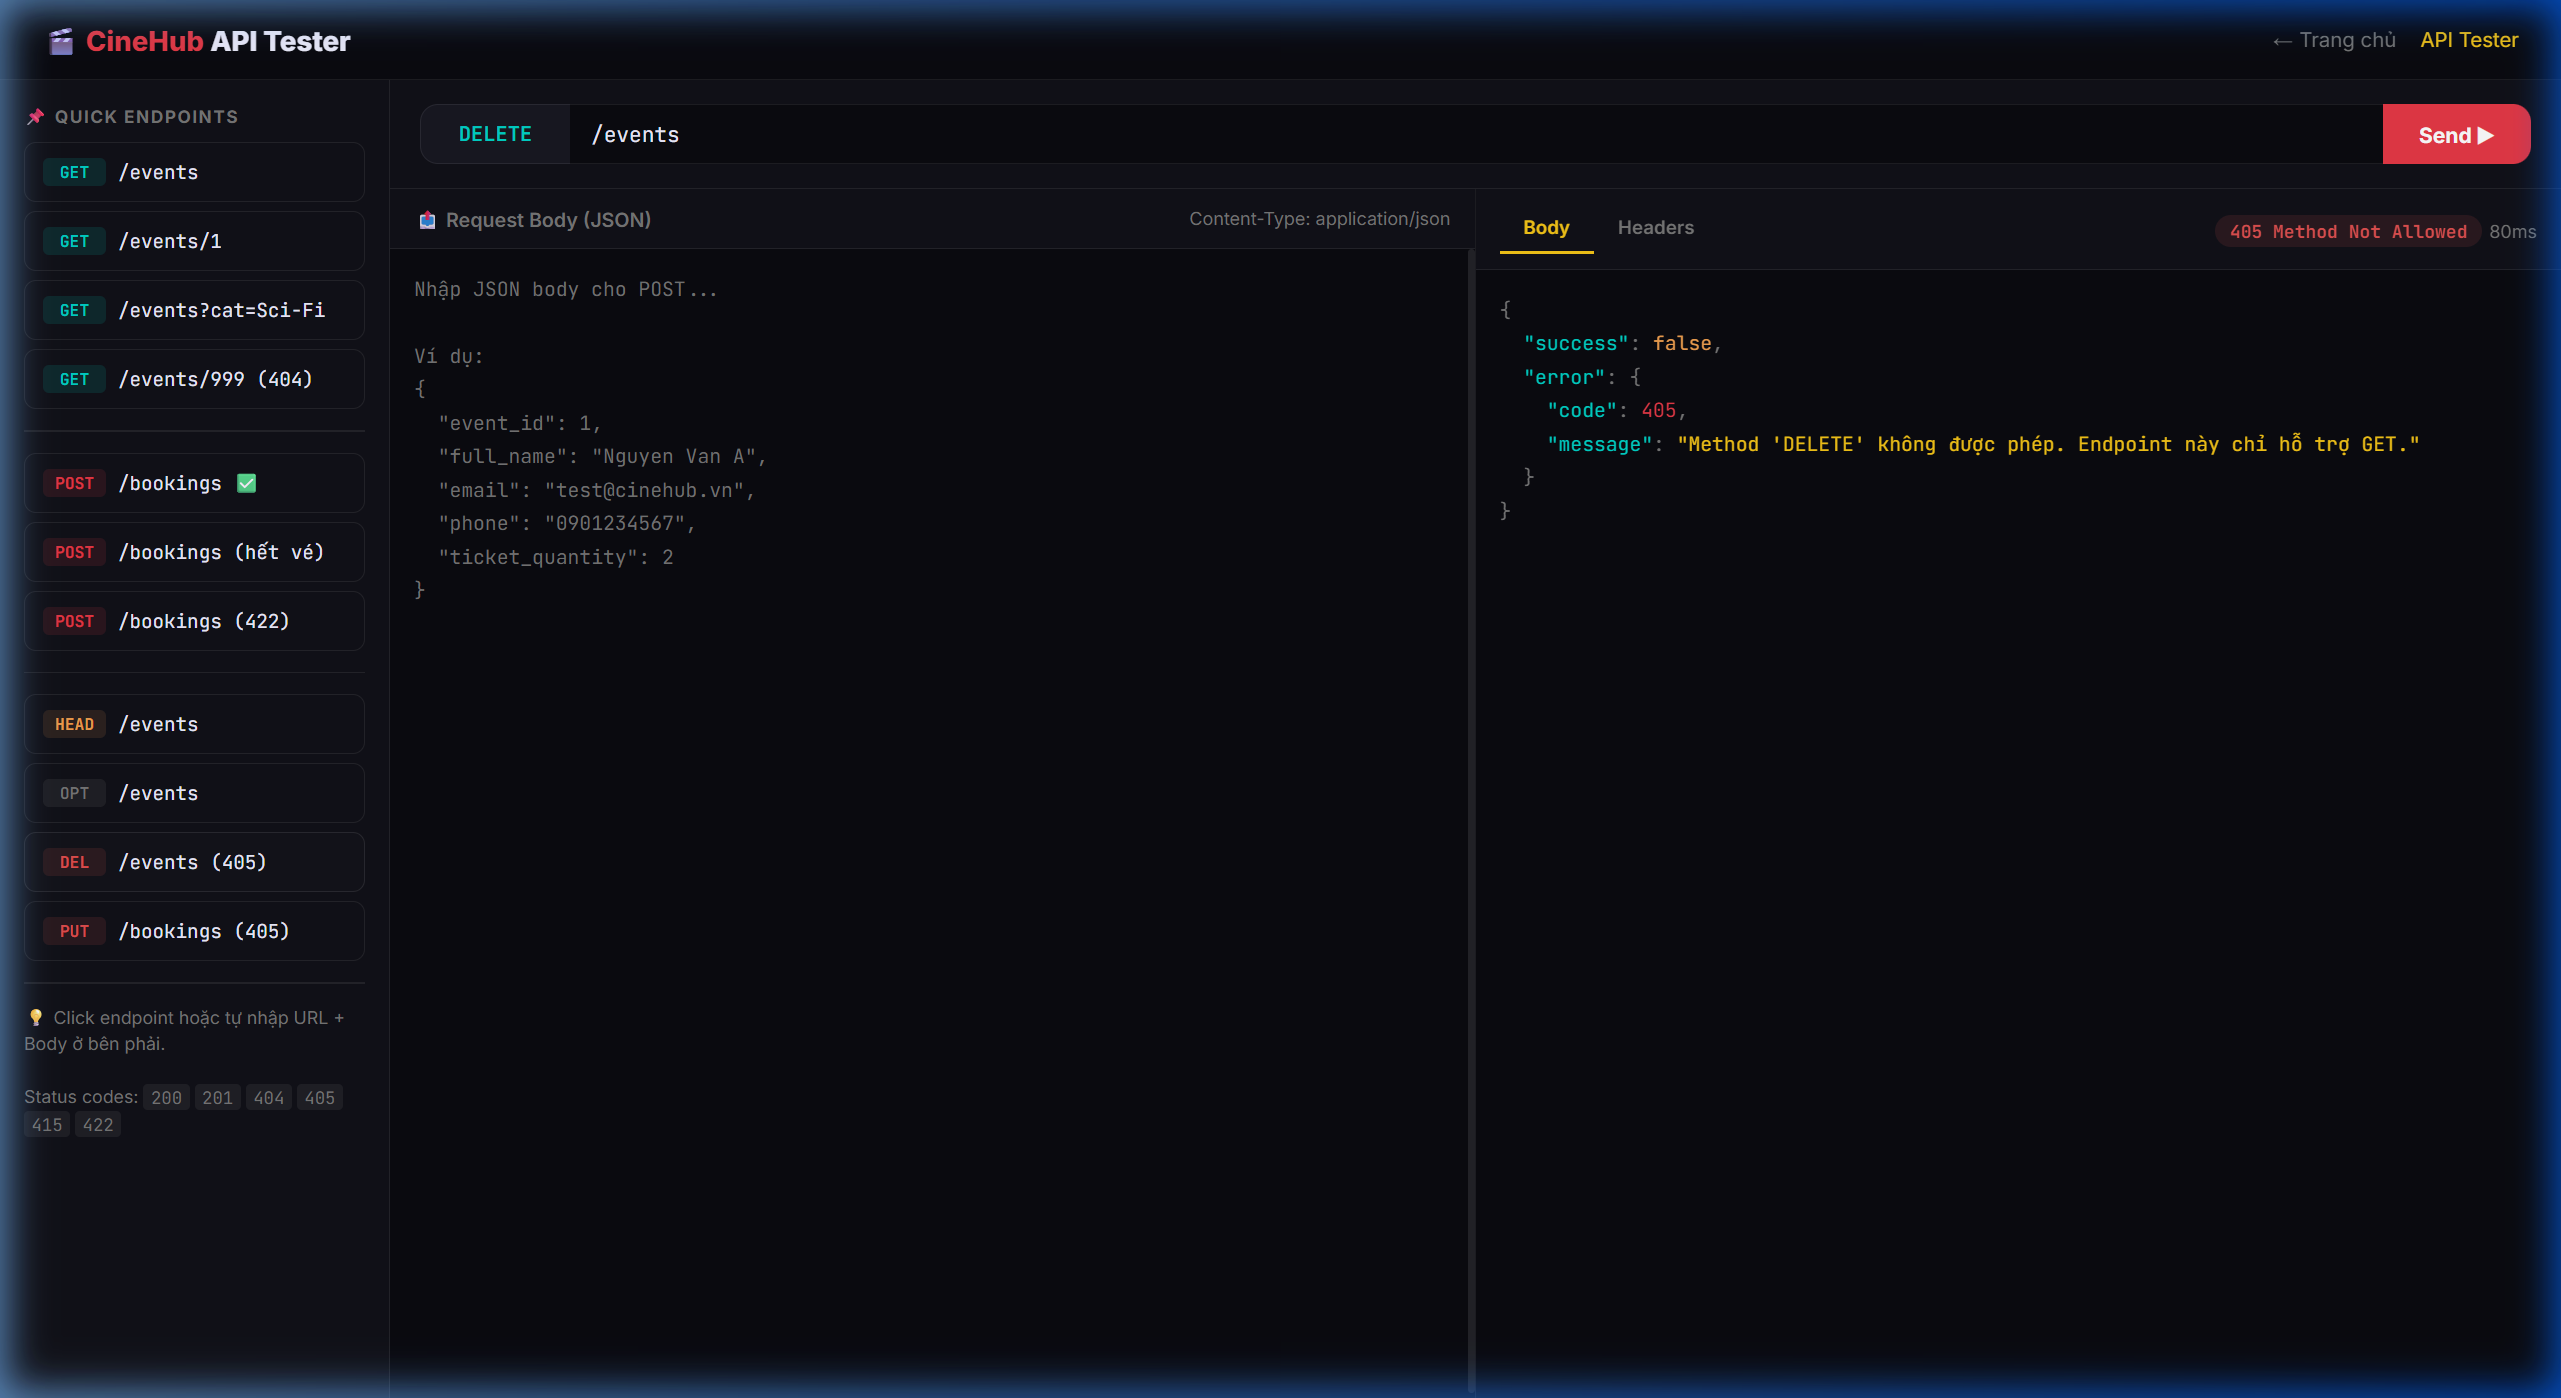
\includegraphics[width=\textwidth]{images/09-del-405.png}
    \caption{DELETE /events — Trả về 405 Method Not Allowed}
\end{figure}

\textbf{415 Unsupported Media Type} — Khi gửi POST không có \texttt{Content-Type: application/json}, hệ thống trả về 415.

\subsubsection{HEAD và OPTIONS}

\begin{itemize}[noitemsep]
    \item \texttt{HEAD /events}: Trả về 200 OK với headers \texttt{X-Total-Events}, \texttt{X-API-Version} nhưng không có body.
    \item \texttt{OPTIONS /events}: Trả về 204 No Content với header \texttt{Allow: GET, POST, HEAD, OPTIONS}.
\end{itemize}

\subsection{Trang API Tester}

Để kiểm tra tất cả endpoint một cách trực quan, em xây dựng thêm trang \textbf{API Tester} (kiểu Postman) tại \texttt{/public/api-tester.html}:

\begin{figure}[H]
    \centering
    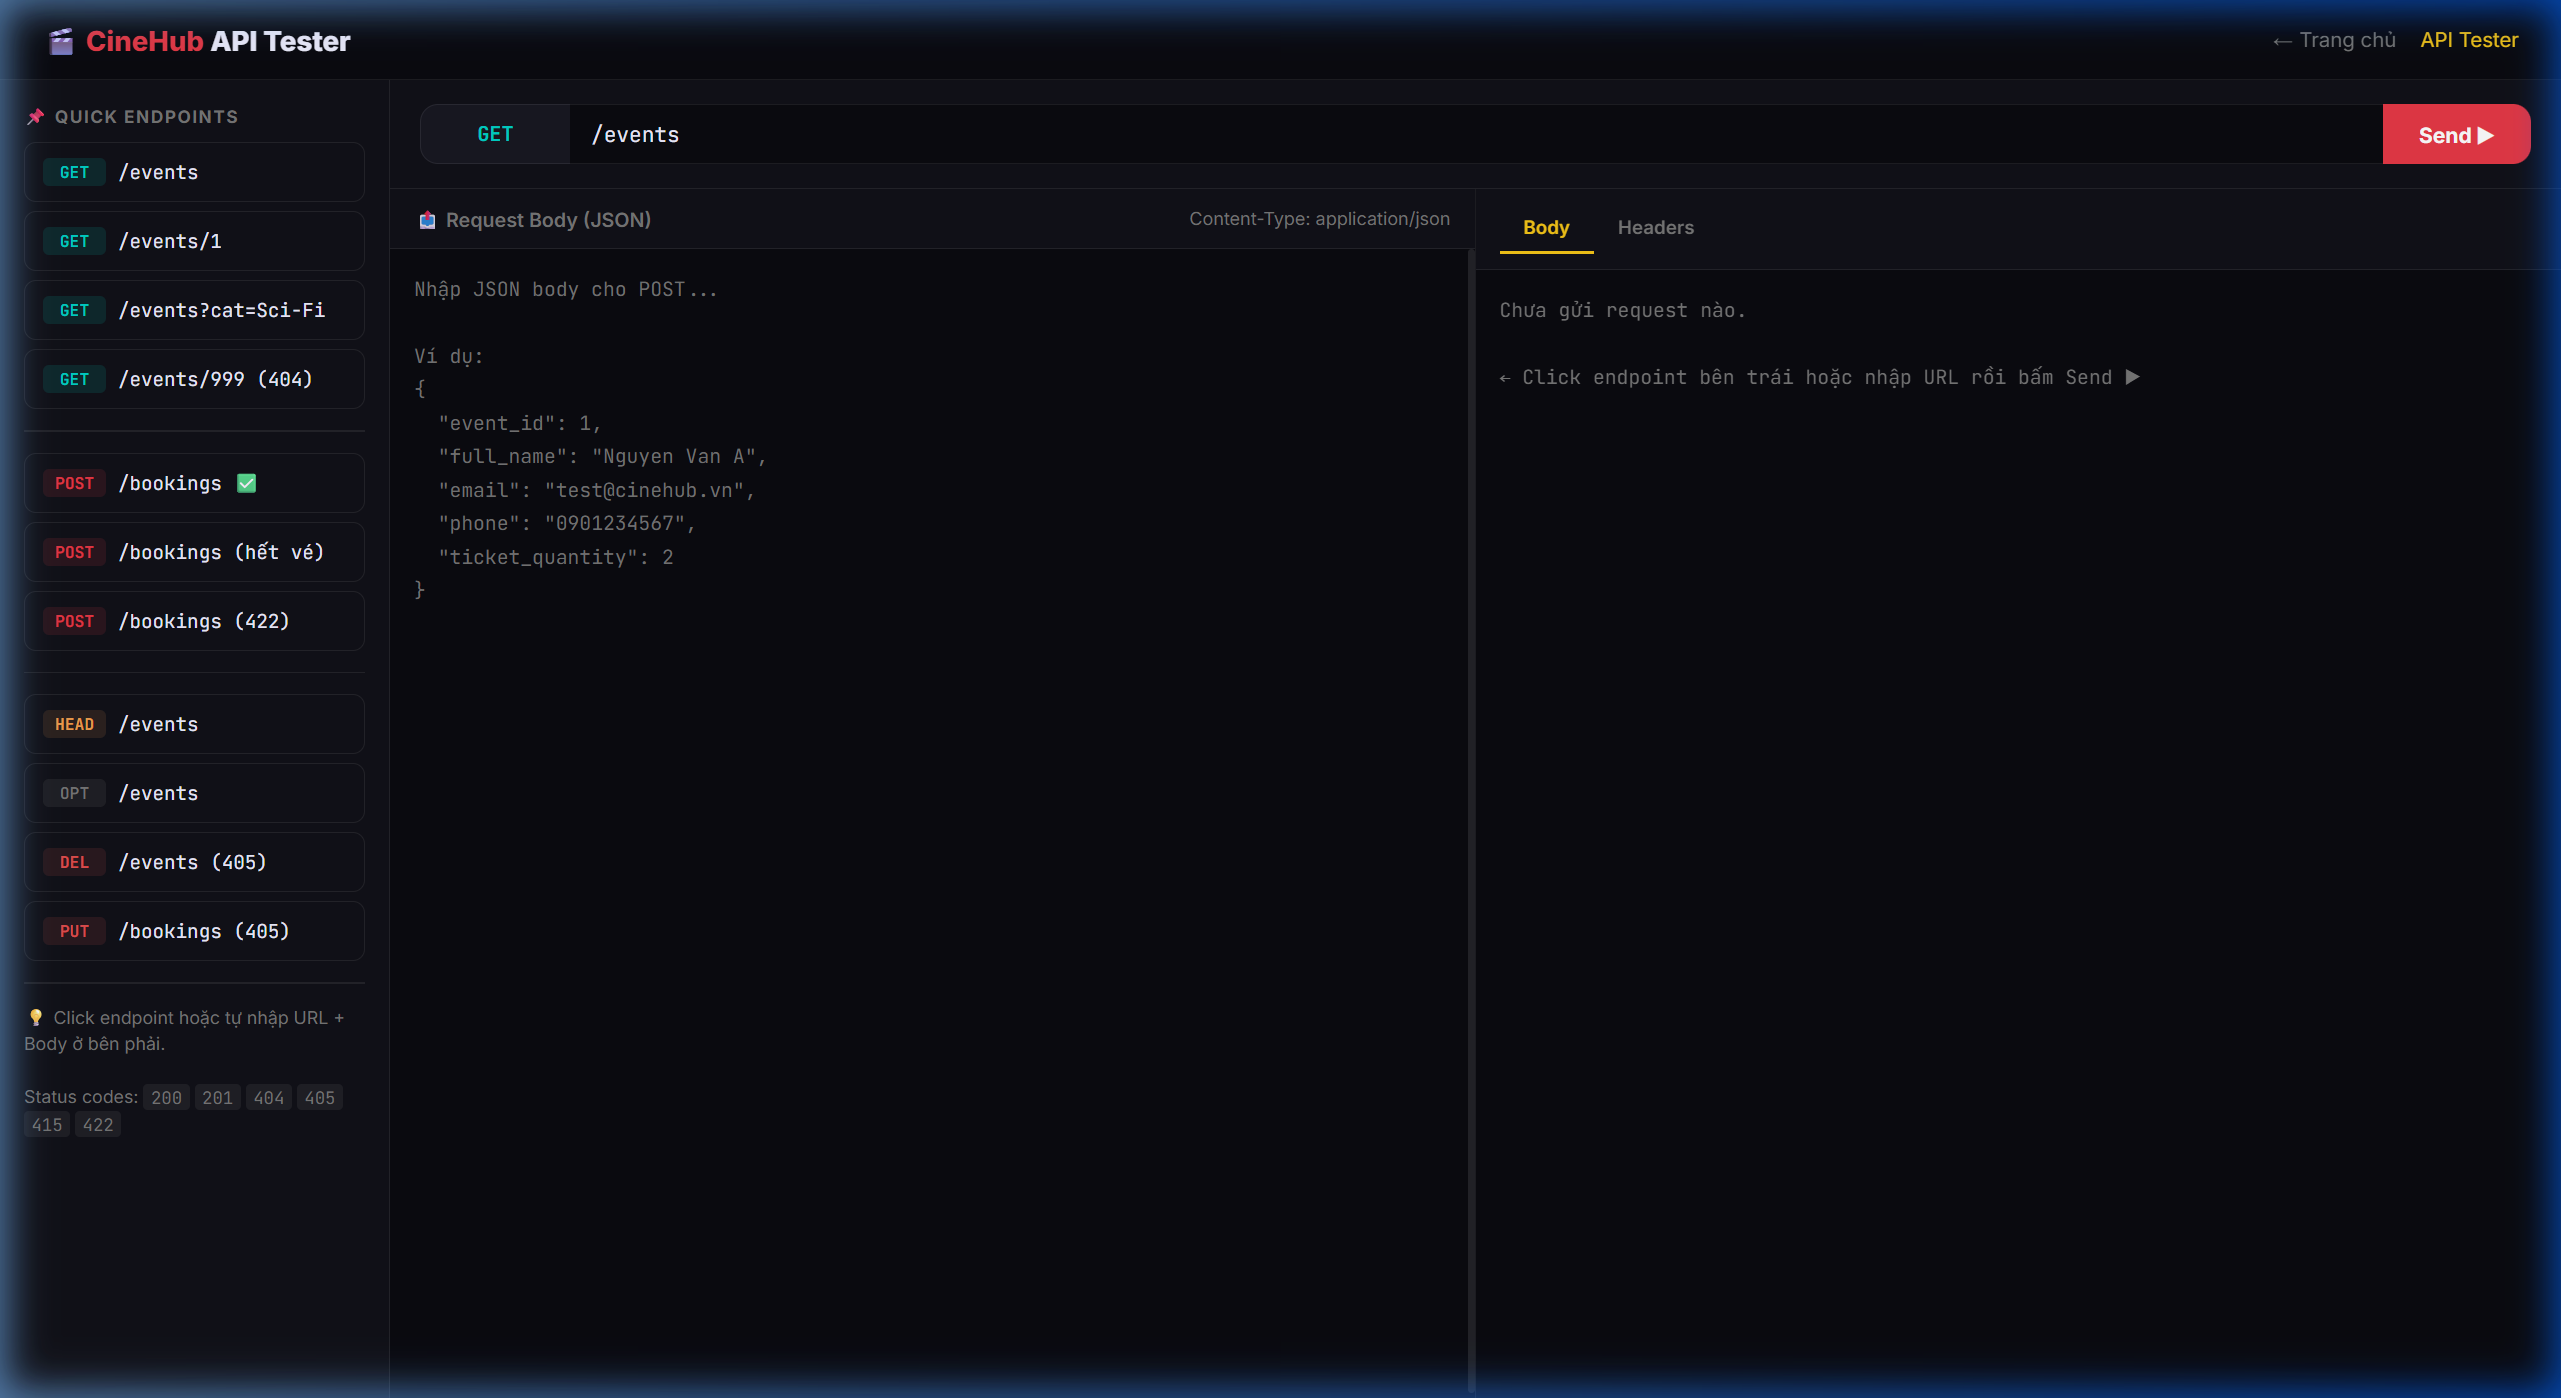
\includegraphics[width=\textwidth]{images/04-api-tester.png}
    \caption{Trang API Tester — giao diện kiểu Postman cho test endpoint}
\end{figure}

Trang API Tester cho phép:
\begin{itemize}[noitemsep]
    \item Chọn HTTP method (GET, POST, HEAD, OPTIONS, PUT, DELETE, PATCH)
    \item Nhập URL và JSON body tùy ý
    \item 11 quick endpoints preset ở sidebar
    \item Xem response JSON syntax-highlighted + response headers
    \item Hiển thị status code (200, 201, 404, 405, 415, 422) + thời gian response
\end{itemize}

\subsection{Quản lý Source Code}

\begin{itemize}[noitemsep]
    \item Git repository: \url{https://github.com/lphhien112-gif/PHP-}
    \item File \texttt{.gitignore}: Bỏ qua \texttt{vendor/}, \texttt{.env}, \texttt{storage/logs/}, và các file LaTeX compiled (\texttt{*.aux, *.log, *.pdf}).
    \item Commit messages mô tả rõ ràng từng tính năng.
\end{itemize}

\subsection{Tóm tắt các yêu cầu đã thực hiện}

\begin{center}
\begin{tabular}{|l|c|}
\hline
\textbf{Yêu cầu} & \textbf{Trạng thái} \\
\hline
Kiểm tra PHP, Composer, Git & \checkmark \\
Cấu trúc thư mục chuẩn (public/, src/, views/, config/, storage/) & \checkmark \\
PSR-4 autoload qua composer.json & \checkmark \\
File .env và .env.example & \checkmark \\
Config đọc biến môi trường & \checkmark \\
Dữ liệu mẫu bằng array PHP (10 phim) & \checkmark \\
Controller / Helper / Support class & \checkmark \\
Entry point tại public/index.php & \checkmark \\
Trang chủ giao diện đặt vé & \checkmark \\
GET endpoint danh sách dữ liệu & \checkmark \\
POST endpoint đặt vé/đăng ký & \checkmark \\
Xử lý sai method (405) & \checkmark \\
Xử lý sai Content-Type (415) & \checkmark \\
Xử lý dữ liệu không hợp lệ (422) & \checkmark \\
Status codes: 200, 201, 404, 405, 415, 422 & \checkmark \\
HEAD và OPTIONS methods & \checkmark \\
Git + GitHub & \checkmark \\
\hline
\end{tabular}
\end{center}

\newpage

% =====================================================
% CÂU 2: PROBLEM SOLVING
% =====================================================
\section{Câu 2: Problem Solving}

\subsection{Câu 2.1 — Hạn chế khi lưu dữ liệu bằng array PHP}

Hiện tại CineHub lưu 10 bộ phim trong mảng \texttt{\$events} ở \texttt{EventController.php}. Nếu tiếp tục phát triển, hệ thống sẽ gặp các hạn chế sau:

\begin{itemize}
    \item \textbf{Cập nhật dữ liệu:} Mỗi lần POST đặt vé, trường \texttt{booked} cần tăng lên — nhưng vì dữ liệu nằm trong array PHP, nó sẽ \textbf{reset về giá trị ban đầu} mỗi khi request mới đến. Ví dụ: phim ``Stellar Frontier'' có \texttt{booked=42}, sau khi đặt 2 vé vẫn hiện 42 ở request tiếp theo.

    \item \textbf{Tìm kiếm:} Khi danh sách phim tăng lên 1000+ bản ghi, việc \texttt{array\_filter()} hoặc loop toàn bộ mảng sẽ rất chậm. Database có index giúp tìm kiếm O(log n) thay vì O(n).

    \item \textbf{Mở rộng bản ghi:} Array PHP nằm trong bộ nhớ RAM — nếu có 10.000 phim với poster, dữ liệu sẽ chiếm rất nhiều memory mỗi request. Database lưu trên disk và chỉ load phần cần thiết.

    \item \textbf{Đồng bộ nhiều người:} Nếu 2 người cùng đặt vé phim ``The Hollow'' (còn 8 ghế) cùng lúc, cả hai đều thấy ``còn 8 ghế'' và cả hai đều đặt thành công — dẫn đến \textbf{overselling}. Database hỗ trợ transaction và locking để tránh race condition này.
\end{itemize}

\subsection{Câu 2.2 — Bổ sung validation cho POST endpoint}

Hiện tại \texttt{EventController::book()} kiểm tra:
\begin{itemize}[noitemsep]
    \item Có đủ 5 trường bắt buộc (\texttt{event\_id, full\_name, email, phone, ticket\_quantity})
    \item \texttt{event\_id} có tồn tại không
    \item Phim còn ghế hay hết
\end{itemize}

\textbf{Cần bổ sung thêm:}
\begin{enumerate}[noitemsep]
    \item \textbf{Định dạng email:} Dùng \texttt{filter\_var(\$email, FILTER\_VALIDATE\_EMAIL)} — hiện tại ``abc123'' vẫn được chấp nhận làm email.
    \item \textbf{Kiểm tra số điện thoại:} Regex \texttt{/\^{}0[0-9]\{9\}\$/} để đảm bảo 10 chữ số bắt đầu bằng 0.
    \item \textbf{Chống trùng đăng ký:} Kiểm tra cùng email + cùng event\_id đã đặt chưa, tránh đặt vé trùng lặp.
    \item \textbf{Giới hạn số vé:} \texttt{ticket\_quantity} phải \texttt{>= 1} và \texttt{<= seats\_left}. Hiện nếu còn 3 ghế mà đặt 5 vẫn có thể thành công.
    \item \textbf{Kiểm tra kiểu dữ liệu:} \texttt{event\_id} và \texttt{ticket\_quantity} phải là số nguyên dương, không phải string ``abc''.
    \item \textbf{Sanitize input:} Dùng \texttt{htmlspecialchars()} cho \texttt{full\_name} để chống XSS injection.
\end{enumerate}

\subsection{Câu 2.3 — Tại sao cần phân biệt rõ status code?}

Thay vì luôn trả \texttt{200} hoặc \texttt{500}, việc dùng đúng mã lỗi (404, 405, 415, 422) mang lại lợi ích cụ thể:

\begin{itemize}
    \item \textbf{Frontend:} Trang CineHub dùng \texttt{fetch()} bắt status code để hiện đúng thông báo. Nếu \texttt{422} → hiện lỗi validation (``Thiếu họ tên''), nếu \texttt{201} → hiện toast ``Đặt vé thành công!''. Nếu luôn trả 200, frontend phải parse body mới biết lỗi hay thành công — dễ bỏ sót.

    \item \textbf{Người dùng:} Mã \texttt{404} cho biết ``phim không tồn tại'' — khác hoàn toàn với \texttt{422} ``thiếu thông tin''. Người dùng biết cần sửa gì thay vì chỉ thấy ``Có lỗi xảy ra''.

    \item \textbf{Debugging:} Khi xem log (\texttt{storage/logs/app.log}), thấy \texttt{405 DELETE /events} ngay lập tức biết có ai đó gọi sai method. Nếu tất cả là 200, phải đọc chi tiết body mới hiểu.

    \item \textbf{Mở rộng API:} Khi thêm mobile app hoặc đối tác tích hợp API, họ chỉ cần dựa vào status code chuẩn HTTP để xử lý — không cần đọc tài liệu format error riêng của CineHub.
\end{itemize}

\subsection{Câu 2.4 — Tại sao cần tách config, .env, source code, log?}

Trong CineHub, các file được tách rõ:
\begin{itemize}[noitemsep]
    \item \texttt{.env} — Biến môi trường (APP\_NAME, APP\_DEBUG)
    \item \texttt{config/app.php} — Logic đọc config
    \item \texttt{src/} — Business logic (Controller, Helper)
    \item \texttt{storage/logs/app.log} — Log hệ thống
\end{itemize}

\textbf{Lý do tách:}

\begin{enumerate}
    \item \textbf{Bảo mật:} File \texttt{.env} chứa thông tin nhạy cảm (sau này có DB password, API key). Nếu viết chung vào \texttt{index.php}, ai có source code là có hết mật khẩu. Tách ra + \texttt{.gitignore} đảm bảo không push lên GitHub.

    \item \textbf{Dễ deploy:} Trên server production, chỉ cần thay \texttt{.env} (APP\_DEBUG=false) mà không sửa code. Trên dev dùng \texttt{APP\_DEBUG=true} để hiện lỗi chi tiết.

    \item \textbf{Log riêng:} File \texttt{app.log} ghi mọi request/error — nếu ghi chung vào source code sẽ rất rối. Tách ra cho phép dùng tool (tail, grep) để monitor realtime.

    \item \textbf{Teamwork:} Nhiều dev làm chung, mỗi người có \texttt{.env} riêng (database local khác nhau). Source code giống nhau nhưng config khác — chỉ hoạt động khi tách file.
\end{enumerate}

\subsection{Câu 2.5 — Ưu tiên mở rộng phần nào trước?}

Em ưu tiên theo thứ tự:

\begin{enumerate}
    \item \textbf{Kết nối database (MySQL):} Đây là \textbf{ưu tiên số 1} vì giải quyết ngay hạn chế lớn nhất (Câu 2.1): dữ liệu booking bị mất khi refresh, không thể cập nhật số ghế thật, race condition khi nhiều người đặt cùng lúc. CineHub hiện có 10 phim cố định — chuyển sang MySQL là bước đầu tiên để hệ thống hoạt động thực tế.

    \item \textbf{Thêm/sửa/xóa dữ liệu (CRUD):} Sau khi có database, cần hoàn thiện CRUD để admin quản lý phim — thêm phim mới, cập nhật lịch chiếu, xóa suất đã hết hạn. Hiện tại muốn thêm phim phải sửa code PHP.

    \item \textbf{Router tốt hơn:} Hiện \texttt{index.php} dùng \texttt{if-else} phân luồng — với 10+ endpoint sẽ rất khó quản lý. Cần router pattern matching (kiểu \texttt{/events/\{id\}}) để code sạch hơn.

    \item \textbf{Validation tốt hơn:} Tạo lớp \texttt{Validator} riêng thay vì validate inline trong controller. Tái sử dụng cho mọi endpoint.

    \item \textbf{Đăng nhập / phân quyền:} Phân biệt admin (quản lý phim) và user (đặt vé). Nhưng chỉ cần thiết khi đã có database và CRUD hoạt động.

    \item \textbf{Logging / monitoring:} Hiện đã có \texttt{Logger.php} cơ bản ghi vào \texttt{app.log}. Nâng cấp thêm log level (info/warning/error) và dashboard monitoring sau cùng.
\end{enumerate}

\textbf{Tóm lại:} Database → CRUD → Router → Validation → Auth → Monitoring. Thứ tự này đảm bảo mỗi bước đều xây trên nền tảng của bước trước.

\newpage

% =====================================================
% KẾT LUẬN
% =====================================================
\section{Kết luận}

Bài thực hành Lab02 đã giúp em hiểu sâu hơn về:
\begin{itemize}[noitemsep]
    \item Cách xây dựng RESTful API hoàn chỉnh với PHP thuần (không framework).
    \item Xử lý đúng các HTTP methods: GET, POST, HEAD, OPTIONS.
    \item Trả về đúng status codes: 200, 201, 404, 405, 415, 422.
    \item Cấu trúc dự án chuẩn PSR-4 với Composer autoload.
    \item Tách biệt config, env, source code, log.
\end{itemize}

\textbf{Điểm nổi bật (làm thêm):}
\begin{itemize}[noitemsep]
    \item Giao diện trang chủ thiết kế chuẩn production (dark-mode, glassmorphism, poster phim AI).
    \item 10 bộ phim với poster sinh bởi AI, đầy đủ metadata.
    \item Trang \textbf{API Tester} kiểu Postman cho phép test mọi endpoint trực quan.
    \item Booking modal với preview phim (thumbnail + thông tin + giá).
    \item Promo banner, filter theo 10 thể loại, animated stats.
    \item Logging mọi request vào \texttt{storage/logs/app.log}.
\end{itemize}

\end{document}
